\documentclass[11pt,a4paper,twoside,openright]{book}
% Shared preamble for the Integration training sheet.
\usepackage[T1]{fontenc}
\usepackage[utf8]{inputenc}
\usepackage{lmodern}
\ifdefined\KindleEdition
  % 6-inch e-ink page (Kindle Paperwhite): the page *is* the screen, so the
  % margins are only what the eye needs, not what a printer needs.
  \usepackage[paperwidth=90mm,paperheight=122mm,
              top=4mm,bottom=6mm,left=4.5mm,right=4.5mm]{geometry}
\else
  \usepackage[a4paper,margin=2.4cm]{geometry}
\fi
\usepackage{amsmath,amssymb,amsthm}
\usepackage{microtype}
\usepackage{enumitem}
\usepackage{xcolor}
\usepackage[most]{tcolorbox}
\usepackage{fancyhdr}
\usepackage[hidelinks]{hyperref}

\definecolor{accent}{HTML}{1F4E79}
\definecolor{soft}{HTML}{F4F7FA}

% --- function graphs ------------------------------------------------------
\usepackage{pgfplots}
\pgfplotsset{compat=1.18}
\usetikzlibrary{arrows.meta}

% One consistent look for every function graph in these books.
\pgfplotsset{
  fnaxis/.style={
    width=5.9cm, height=4.6cm,
    axis lines=middle,
    axis line style={-{Stealth[length=4pt]}, gray!65!black, line width=0.3pt},
    tick style={gray!65!black},
    tick label style={font=\tiny, gray!50!black},
    label style={font=\scriptsize},
    xlabel={$x$}, ylabel={$y$},
    every axis x label/.style={at={(ticklabel* cs:1.0)}, anchor=west},
    every axis y label/.style={at={(ticklabel* cs:1.0)}, anchor=south east,
      xshift=-1pt},
    every axis plot/.append style={accent, very thick, smooth, samples=201},
    clip=true, enlargelimits=false,
    title style={font=\scriptsize, yshift=4pt},
  },
  fnaxis/.append style={/pgfplots/legend style={font=\tiny, draw=none,
    fill=none, at={(0.98,0.03)}, anchor=south east}},
}

% A row of small graphs, evenly spaced with \hfill between them, plus an
% optional caption line: \begin{gallery} <pic>\hfill<pic> \gcap{...} \end{gallery}
\newenvironment{gallery}
  {\par\medskip\noindent\ignorespaces}
  {\par\medskip\noindent}
\newcommand{\gcap}[1]{\par\smallskip{\centering\footnotesize #1\par}}

% --- plane regions, implicit curves, surfaces -----------------------------
\usepgfplotslibrary{fillbetween}
\definecolor{regionfill}{HTML}{9DB4D8}
\pgfplotsset{colormap={house}{color=(soft) color=(accent!45) color=(accent)}}

\pgfplotsset{
  % Squared, gridded axis for plane regions and implicitly given curves.
  geoaxis/.style={
    fnaxis,
    width=5.9cm, height=5.9cm,
    grid=both,
    grid style={gray!22, line width=0.2pt},
    minor tick num=1,
  },
  % Level-curve maps: many thin curves, no single curve emphasised.
  contouraxis/.style={
    geoaxis,
    every axis plot/.append style={accent!75, line width=0.5pt, smooth,
      samples=201},
  },
  % Surfaces: \addplot3[surf, domain=..., y domain=...] {expr};
  surfaxis/.style={
    width=6.0cm, height=5.0cm,
    view={130}{22},
    colormap name=house,
    ticks=none,
    xlabel={$x$}, ylabel={$y$}, zlabel={$f$},
    label style={font=\tiny, gray!50!black},
    title style={font=\scriptsize},
    every axis plot/.append style={samples=25, shader=faceted interp,
      draw=accent!35, line width=0.1pt},
  },
}

% Shorthand for a shaded region between two named paths.
% \region{<path A>}{<path B>}{<soft clip options>}
\newcommand{\region}[3]{%
  \addplot[regionfill, opacity=0.55, forget plot, sharp plot]
    fill between[of=#1 and #2, #3];}

% --- rule boxes -----------------------------------------------------------
\newtcolorbox{rulebox}[1]{%
  breakable, enhanced, colback=soft, colframe=accent,
  boxrule=0.4pt, left=7pt, right=7pt, top=6pt, bottom=6pt,
  fonttitle=\bfseries, coltitle=white, colbacktitle=accent,
  title={#1}}

% --- worked examples ------------------------------------------------------
% One fully narrated solution per chapter, carrying the chapter's central
% technique and the mistakes that technique invites:
%   \begin{worked}{Task} ... \wstep{Step 1.} ... \wtrap{...} ... \end{worked}
\newtcolorbox{worked}[1]{%
  breakable, enhanced, colback=white, colframe=accent!65,
  boxrule=0.4pt, left=7pt, right=7pt, top=6pt, bottom=6pt,
  fonttitle=\bfseries, coltitle=accent, colbacktitle=soft,
  title={#1}}

% Run-in step heading inside a worked example.
\newcommand{\wstep}[1]{\par\smallskip\noindent\textbf{#1}\enspace\ignorespaces}

% A pitfall, set off from the running solution so it can be found again.
\newcommand{\wtrap}[1]{%
  \par\smallskip
  {\leftskip=1.3em\noindent
   \llap{\textcolor{accent}{\rule[0.22ex]{0.9em}{0.6pt}}\hspace{0.4em}}%
   \textbf{Trap.}\enspace\itshape #1\par}%
  \smallskip}

% --- problem / solution lists --------------------------------------------
\newlist{problems}{enumerate}{1}
\setlist[problems]{label=\textbf{\arabic*.}, leftmargin=2.1em,
  itemsep=0.55ex, parsep=0pt, topsep=0.8ex}
\newlist{solutions}{enumerate}{1}
\setlist[solutions]{label=\textbf{\arabic*.}, leftmargin=2.1em,
  itemsep=1.0ex, parsep=0pt, topsep=0.8ex}

% --- running heads --------------------------------------------------------
\pagestyle{fancy}
\fancyhf{}
\fancyhead[LE,RO]{\thepage}
\fancyhead[RE]{\small\itshape\nouppercase{\leftmark}}
\fancyhead[LO]{\small\itshape\nouppercase{\rightmark}}
\setlength{\headheight}{14pt}
\renewcommand{\headrulewidth}{0.3pt}
\renewcommand{\chaptermark}[1]{\markboth{\chaptername\ \thechapter.\ #1}{}}
\renewcommand{\sectionmark}[1]{\markright{\thesection\ #1}}

% --- shorthands used throughout -------------------------------------------
\newcommand{\dd}[2]{\frac{\mathrm{d}#1}{\mathrm{d}#2}}
\newcommand{\pd}[2]{\frac{\partial #1}{\partial #2}}
\newcommand{\pdd}[3]{\frac{\partial^{2} #1}{\partial #2\,\partial #3}}
\newcommand{\R}{\mathbb{R}}
\newcommand{\grad}{\nabla}
\DeclareMathOperator{\sgn}{sgn}
\DeclareMathOperator{\Hess}{H}

% German gloss, used on first mention of a technical term
\newcommand{\de}[1]{\emph{#1}}

% --- cross-references to chapters ------------------------------------------
% Chapter files are shared by the standalone volumes and the compendium, so a
% hard-coded "Chapter 6" is wrong in one of them. Write \chref{derivatives}{6}
% instead: it prints "Chapter 6" inside the same volume, "Volume 5, Chapter 6"
% from another volume, and the running number ("Chapter 34") in the
% compendium. \chrefs{vol}{n} is the abbreviated form (Ch. / Vol., Ch.),
% \chnum{vol}{n} the bare number in the current build, and \volref{vol} names
% the volume ("Volume 5", or "Part V" in the compendium). Each volume's
% main.tex sets \thisvolume; the compendium's sets \incompendiumtrue.
\newif\ifincompendium
\newcommand*{\thisvolume}{}
\makeatletter
\@namedef{chref@vol@algebra}{1}\@namedef{chref@off@algebra}{0}
\@namedef{chref@vol@functions}{2}\@namedef{chref@off@functions}{9}
\@namedef{chref@vol@matrices}{3}\@namedef{chref@off@matrices}{14}
\@namedef{chref@vol@foundations}{4}\@namedef{chref@off@foundations}{24}
\@namedef{chref@vol@derivatives}{5}\@namedef{chref@off@derivatives}{28}
\@namedef{chref@vol@integrals}{6}\@namedef{chref@off@integrals}{42}
\@namedef{chref@vol@optimization}{7}\@namedef{chref@off@optimization}{50}
\@namedef{chref@vol@linprog}{8}\@namedef{chref@off@linprog}{60}
\@namedef{chref@vol@mixed}{9}\@namedef{chref@off@mixed}{68}
\newcommand*{\chref@check}[1]{%
  \@ifundefined{chref@vol@#1}{\PackageError{chref}{Unknown volume `#1'}{}}{}}
\newcommand*{\chnum}[2]{\chref@check{#1}%
  \ifincompendium\the\numexpr\csname chref@off@#1\endcsname+#2\relax
  \else#2\fi}
% \chref@same{vol}{same volume}{other volume}
\newcommand*{\chref@same}[3]{\def\chref@tmp{#1}%
  \ifx\chref@tmp\thisvolume\expandafter\@firstoftwo
  \else\expandafter\@secondoftwo\fi{#2}{#3}}
\newcommand*{\chref}[2]{\chref@check{#1}%
  \ifincompendium Chapter~\chnum{#1}{#2}%
  \else\chref@same{#1}{Chapter~#2}%
    {Volume~\csname chref@vol@#1\endcsname, Chapter~#2}\fi}
\newcommand*{\chrefs}[2]{\chref@check{#1}%
  \ifincompendium Ch.~\chnum{#1}{#2}%
  \else\chref@same{#1}{Ch.~#2}%
    {Vol.~\csname chref@vol@#1\endcsname, Ch.~#2}\fi}
\newcommand*{\volref}[1]{\chref@check{#1}%
  \ifincompendium Part~\@Roman{\csname chref@vol@#1\endcsname}%
  \else Volume~\csname chref@vol@#1\endcsname\fi}
\makeatother

% --- Kindle edition: compact layout for a 6-inch screen -------------------
% Everything below applies only when \KindleEdition is defined on the
% command line; the A4 edition is untouched.
\ifdefined\KindleEdition
  \usepackage{etoolbox}
  \usepackage{adjustbox}
  \usepackage{titlesec}

  % The 8cm measure leaves few break points; let TeX loosen a tight line
  % rather than push it into the margin.
  \setlength{\emergencystretch}{1.5em}

  % No running heads: on a 90mm page the header costs more than it gives.
  % A centred page number in the foot is kept so the contents list means
  % something.
  \pagestyle{plain}
  \fancypagestyle{plain}{\fancyhf{}\fancyfoot[C]{\small\thepage}%
    \renewcommand{\headrulewidth}{0pt}}

  % Compact headings: the book class leaves a third of a page above a
  % chapter title, which is unaffordable here.
  \titleformat{\chapter}[display]
    {\normalfont\Large\bfseries\color{accent}}{\normalsize\chaptertitlename\ \thechapter}{0.4em}{\Large}
  \titlespacing*{\chapter}{0pt}{0pt}{1.2em}
  \titlespacing*{\section}{0pt}{1.4ex plus .3ex}{0.7ex}
  \titlespacing*{\subsection}{0pt}{1.2ex plus .2ex}{0.5ex}

  % Boxes: trim the padding, which was set for a 16cm measure.
  \tcbset{left=3.5pt,right=3.5pt,top=3pt,bottom=3pt,
          fonttitle=\bfseries\small,
          halign title=flush left}

  % Problem and solution lists: reclaim the wide left margin.
  \setlist[problems]{label=\textbf{\arabic*.}, leftmargin=1.5em,
    itemsep=0.45ex, parsep=0pt, topsep=0.6ex}
  \setlist[solutions]{label=\textbf{\arabic*.}, leftmargin=1.5em,
    itemsep=0.8ex, parsep=0pt, topsep=0.6ex}

  % Figures and wide tables shrink to the measure instead of running off it.
  % adjustbox only scales down: anything already narrow is left alone.
  \BeforeBeginEnvironment{tikzpicture}{\begin{adjustbox}{max width=\linewidth}}
  \AfterEndEnvironment{tikzpicture}{\end{adjustbox}}
  \BeforeBeginEnvironment{tabular}{\begin{adjustbox}{max width=\linewidth}}
  \AfterEndEnvironment{tabular}{\end{adjustbox}}

  % Display maths was written for a 16cm measure. On 8cm the long chained
  % equations would run off the screen, so any display wider than the text
  % block is scaled down to fit; narrower ones are left at full size. The
  % whole corpus uses \[ ... \] and no other display environment, so this
  % one redefinition covers every case.
  \newsavebox{\kndbox}
  \renewcommand{\[}{\par\addvspace{0.7ex}%
    \begin{lrbox}{\kndbox}$\displaystyle}
  \renewcommand{\]}{$\end{lrbox}%
    {\centering
      \ifdim\wd\kndbox>\linewidth
        \resizebox{\linewidth}{!}{\usebox{\kndbox}}%
      \else
        \usebox{\kndbox}%
      \fi
     \par}%
    \addvspace{0.7ex}}

  % A narrow measure makes perfect justification impossible; prefer a loose
  % line to a line that runs into the margin.
  \sloppy
  \raggedbottom
\fi


\title{\Huge Algebraic Foundations\\[0.4em]
  \large A Refresher with Exercises and Worked Solutions}
\author{}
\date{}

\begin{document}
\frontmatter
\maketitle

\chapter*{About this sheet}
\addcontentsline{toc}{chapter}{About this sheet}

This is the volume to start with if the algebra has gone rusty. Everything
that follows in the other volumes leans on it: exponents and roots,
logarithms, rational expressions, expanding and factoring, inequalities,
functions with their domains, graphs and transformations, systems of
equations, summation notation, partial fractions, and the algebra of
first-order conditions.

None of it is new mathematics. The point is fluency. A derivative that takes
three lines becomes a derivative that takes one once the exponent rules are
automatic; an integral stops being hard once the partial-fraction step
stops being hard; and the first-order conditions of an optimization problem
are only as tractable as the algebra used to solve them. The last chapter
exists for exactly that reason: it drills the manipulation that every
optimization problem in the later volumes ends up demanding.

Chapters~6 to~8 sit in the middle for the same reason. Before a limit, a
derivative or an optimum can be discussed at all, one has to know where a
function is defined, what values it takes, what its graph looks like, and
how the graph moves when the formula changes. Those three chapters state
the rules, show the standard shapes, and then drill seventy problems
apiece.

Each chapter is thirty-odd problems --- seventy in the three chapters on
functions --- with a fully worked solution for every one, preceded by a
compact statement of the rules being drilled. Work the
problems before reading the solutions; the goal is to make the steps
automatic, and reading someone else's steps does not do that.

\tableofcontents

\mainmatter
\chapter{Exponents and Roots}

Simplify each expression. Assume all variables are positive unless stated
otherwise. Write answers without negative exponents where possible.

\section{Practice Problems}

\begin{problems}
  \item $(x^{2})^{3}\cdot x^{-4}$
  \item $\displaystyle\frac{(2x^{3})^{2}}{4x^{4}}$
  \item $\displaystyle\frac{12a^{5}b^{2}}{4a^{3}b^{7}}$
  \item $\displaystyle\left(\frac{x^{4}y^{-2}}{x\,y^{-5}}\right)^{2}$
  \item Simplify $\sqrt{72}$.
  \item Evaluate $\sqrt[3]{-125}$.
  \item Evaluate $32^{2/5}$.
  \item Evaluate $\displaystyle\left(\frac{16}{81}\right)^{-3/4}$.
  \item $\sqrt[4]{x^{12}y^{8}z^{4}}$
  \item $9^{x/2}\cdot 9^{-x/4}$
  \item $(K^{1/3}L^{2/3})^{3}$
  \item $\displaystyle\frac{\mathrm{e}^{2t}\cdot \mathrm{e}^{-t}}{\mathrm{e}^{3t}}$
  \item $\sqrt{x^{2}}$ for $x\in\R$ (no positivity assumption)
  \item $(0.25)^{-1/2}$
  \item $(a^{1/2}+b^{1/2})(a^{1/2}-b^{1/2})$
  \item $\sqrt[3]{27\,x^{6}y^{-9}}$
  \item $\displaystyle\frac{x^{n+1}}{x^{n-1}}$
  \item $5^{x+1}\cdot 5^{-x}$
  \item Write $\displaystyle\frac{1}{\sqrt[3]{x^{2}}}$ as a single power of $x$.
  \item $\displaystyle\left(\frac{p}{q}\right)^{-n}$
  \item $\displaystyle\frac{(3x^{2})^{2}-(2x)^{2}}{x^{2}}$
  \item $\sqrt{12\,x^{3}y^{4}}$
  \item $\displaystyle\frac{a^{2n}}{a^{n}\cdot a^{n-1}}$
  \item Show that the CES form $(\alpha K^{\rho}+(1-\alpha)L^{\rho})^{1/\rho}$
        reduces to a linear combination when $\rho=1$.
  \item $\displaystyle\frac{2^{n+2}-2^{n+1}}{2^{n}}$
  \item $\left((-3)^{2}\right)^{1/2}$
  \item $\sqrt[5]{x^{15}y^{10}}$
  \item $\displaystyle\frac{(xy^{2})^{3}}{(x^{2}y)^{2}}$
  \item $\displaystyle\sqrt{\frac{9}{16x^{4}}}$
  \item $\displaystyle\frac{8\cdot 2^{n}}{4^{n}}$
\end{problems}

\section{Solutions}

\begin{solutions}
  \item $x^{2}$
  \item $x^{2}$
  \item $\displaystyle\frac{3a^{2}}{b^{5}}$
  \item $x^{6}y^{6}$
  \item $6\sqrt{2}$
  \item $-5$
  \item $4$
  \item $\displaystyle\frac{27}{8}$
  \item $x^{3}y^{2}z$
  \item $9^{x/4}=3^{x/2}$
  \item $KL^{2}$
  \item $\displaystyle\frac{1}{\mathrm{e}^{2t}}$
  \item $|x|$
  \item $2$
  \item $a-b$
  \item $\displaystyle\frac{3x^{2}}{y^{3}}$
  \item $x^{2}$
  \item $5$
  \item $x^{-2/3}$
  \item $\displaystyle\left(\frac{q}{p}\right)^{n}$
  \item $9x^{2}-4$
  \item $2xy^{2}\sqrt{3x}$
  \item $a$
  \item $\alpha K+(1-\alpha)L$ (linear, the Cobb--Douglas exponent limit on
        the simplex)
  \item $2$
  \item $3$
  \item $x^{3}y^{2}$
  \item $\displaystyle\frac{y^{4}}{x}$
  \item $\displaystyle\frac{3}{4x^{2}}$
  \item $2^{3-n}$
\end{solutions}

\chapter{Logarithms and Exponentials}

Mix of evaluating, expanding, condensing, and solving. Bases of 10 and 2
appear alongside the natural log.

\section{Core Rules}

\begin{rulebox}{What a logarithm is}
$\log_{a}(b)$ is \textbf{the exponent that turns $a$ into $b$}:
\[
  \log_{a}(b)=c\iff a^{c}=b\qquad (a>0,\ a\neq1,\ b>0).
\]
Every log identity below is an exponent law read backwards. The domain
restriction $b>0$ is part of the definition, not a technicality: it is what
manufactures extraneous roots when you solve equations.
\end{rulebox}

\begin{rulebox}{The three laws, and the change of base}
\[
  \ln(xy)=\ln x+\ln y,\qquad
  \ln\!\Bigl(\frac{x}{y}\Bigr)=\ln x-\ln y,\qquad
  \ln(x^{p})=p\ln x .
\]
The third is the workhorse: it is what pulls an unknown down out of an
exponent. Any base converts to any other,
\[
  \log_{a}(b)=\frac{\ln b}{\ln a},
\]
so a calculator with only $\ln$ suffices. Also $\ln(\mathrm{e}^{x})=x$ and
$\mathrm{e}^{\ln x}=x$: the two functions undo each other.
\end{rulebox}

\begin{rulebox}{There is no law for a sum inside the log}
\[
  \ln(x+y)\neq\ln x+\ln y .
\]
The left side cannot be expanded at all. The laws convert
\emph{multiplication into addition}, never addition into anything. The same
warning in the other direction: $\ln x\cdot\ln y$ does not simplify, and
$(\ln x)^{2}\neq\ln(x^{2})=2\ln x$.
\end{rulebox}

\begin{rulebox}{Solving: the standard shapes}
\begin{itemize}[leftmargin=1.6em,itemsep=0.3ex]
  \item \textbf{Unknown in the exponent} ($a^{x}=b$): take $\ln$ of both
        sides, then $x=\ln b/\ln a$.
  \item \textbf{Unknown in the base} ($x^{n}=b$): raise both sides to
        $1/n$.
  \item \textbf{Logs on both sides}: condense each side to a single log,
        then drop the logs --- legitimate because $\ln$ is one-to-one.
  \item \textbf{One log, one number}: condense, then exponentiate.
\end{itemize}
Then \textbf{check every root against the original domain.}
\end{rulebox}

\section{Worked Examples}

\begin{worked}{(a) Solve $\log_{3}(x)+\log_{3}(x-2)=1$}
\wstep{Step 1. Record the domain first, before solving anything.}
Both logs must take positive arguments: $x>0$ \emph{and} $x-2>0$, so
\[
  x>2 .
\]
Writing this down now costs one line and settles the last step
automatically.

\wstep{Step 2. Condense the left side to a single logarithm.}
\[
  \log_{3}(x)+\log_{3}(x-2)=\log_{3}\bigl(x(x-2)\bigr).
\]

\wstep{Step 3. Undo the logarithm.}
The equation now reads $\log_{3}\bigl(x(x-2)\bigr)=1$, and by the
definition of a logarithm that says $3^{1}=x(x-2)$:
\[
  x^{2}-2x=3\quad\Longrightarrow\quad x^{2}-2x-3=0
  \quad\Longrightarrow\quad (x-3)(x+1)=0 .
\]

\wstep{Step 4. Apply the domain.}
The candidates are $x=3$ and $x=-1$. The second fails $x>2$ --- indeed
$\log_{3}(-1)$ does not exist --- so
\[
  \boxed{x=3}.
\]
Check: $\log_{3}3+\log_{3}1=1+0=1$. \checkmark
\wtrap{$x=-1$ is not a wrong calculation; it is a genuine root of the
\emph{quadratic}, which is a different equation from the one asked. The
condensing step in Step~2 enlarged the domain, and enlarging a domain is
exactly what creates extraneous roots. Any time you condense two logs into
one, the final domain check is compulsory.}
\end{worked}

\begin{worked}{(b) How long until an economy doubles? Solve $Y_{0}\mathrm{e}^{gt}=2Y_{0}$, and solve $(1+r)^{10}=2$}
\wstep{Step 1. Cancel what is common, then isolate the exponential.}
$Y_{0}>0$, so dividing by it is legal and the initial level drops out
entirely: $\mathrm{e}^{gt}=2$. \emph{Doubling time does not depend on where
you start} --- that is the content of exponential growth, and it is visible
here before any calculation.

\wstep{Step 2. The unknown is in the exponent, so take logs.}
\[
  \ln\bigl(\mathrm{e}^{gt}\bigr)=\ln 2
  \quad\Longrightarrow\quad
  gt=\ln 2
  \quad\Longrightarrow\quad
  t=\frac{\ln 2}{g}\approx\frac{0.693}{g}.
\]
At $g=0.03$ this is $23.1$ years --- the ``rule of 70'', which is just
$100\ln 2\approx69.3$ rounded.

\wstep{Step 3. The second equation has the unknown in the \emph{base}.}
$(1+r)^{10}=2$: here $r$ sits inside the base, not the exponent, so logs
are the wrong tool. Undo the tenth power with a tenth root:
\[
  1+r=2^{1/10}\quad\Longrightarrow\quad r=2^{1/10}-1\approx0.0718 .
\]
So $7.18\%$ a year doubles capital in a decade.
\wtrap{Decide \emph{where the unknown lives} before choosing a move.
Unknown in the exponent $\Rightarrow$ take logs. Unknown in the base
$\Rightarrow$ take a root. Taking logs of $(1+r)^{10}=2$ is not wrong, but
it leads to $\ln(1+r)=\tfrac{1}{10}\ln2$ and one more exponentiation to
undo --- the long way round.}
\end{worked}

\section{Practice Problems}

\begin{problems}
  \item Evaluate: $\ln(1)$
  \item Evaluate: $\log_{10}(100)$
  \item Evaluate: $\log_{2}(32)$
  \item Evaluate: $\ln(\mathrm{e})+\ln(\mathrm{e}^{3})$
  \item Expand: $\displaystyle\ln\left(\frac{x^{a}}{y^{b}z^{c}}\right)$
  \item Expand: $\displaystyle\ln\left(\sqrt[5]{\frac{x^{3}}{y^{2}}}\right)$
  \item Can $\ln(x^{2}+y^{2})$ be expanded? Why?
  \item Expand: $\ln(C\,\mathrm{e}^{-\delta t})$
  \item Condense: $4\ln(x)-2\ln(y)+\tfrac12\ln(z)$
  \item Condense: $\tfrac13\ln(8)+\tfrac12\ln(9)$
  \item Condense: $\ln(a)+\ln(b)-\ln(c)-\ln(d)$
  \item Solve for $x$: $\log_{10}(x)=3$
  \item Solve for $x$ ($x>0$): $\ln(x)=-1$
  \item Solve for $x$ ($x>2$): $\ln(x)+\ln(x-2)=\ln(3)$
  \item Half-life: solve $\tfrac12 P_{0}=P_{0}\,\mathrm{e}^{-\lambda t}$ for
        $t$.
  \item Solve for $r$: $(1+r)^{10}=2$
  \item Solve for $\alpha$ ($0<\alpha<1$): $\ln(\alpha)-\ln(1-\alpha)=1$
  \item Solve for $x$: $\mathrm{e}^{2x}-3\mathrm{e}^{x}+2=0$ (Hint:
        substitute $u=\mathrm{e}^{x}$.)
  \item Solve for $T$: $A=P(1+r)^{T}$
  \item Solve for $x$ ($x>0$): $(\ln x)^{2}=\ln(x^{4})$
  \item Solve for $t$: $A_{0}\cdot 2^{-t/h}=\dfrac{A_{0}}{8}$
  \item Expand: $\displaystyle\ln\left(\frac{(1+r)^{T}}{r}\right)$
  \item Solve: $\log_{3}(x)+\log_{3}(x-2)=1$
  \item Solve: $\log_{2}(x+1)-\log_{2}(x-1)=1$
  \item Solve: $\mathrm{e}^{x}=5\,\mathrm{e}^{-x}$
  \item Solve: $4^{x}=8$
  \item Given $\ln 2\approx 0.693$ and $\ln 3\approx 1.099$, estimate
        $\ln 12$.
  \item Use the change-of-base formula to express $\log_{5}(20)$ as a ratio
        of natural logs.
  \item Solve for $K$ in $\ln(Y)=\ln(A)+\alpha\ln(K)+(1-\alpha)\ln(L)$.
  \item Solve for $g$: $Y_{t}=Y_{0}\,\mathrm{e}^{gt}$
\end{problems}

\section{Solutions}

\begin{solutions}
  \item $0$
  \item $2$
  \item $5$
  \item $1+3=4$
  \item $a\ln(x)-b\ln(y)-c\ln(z)$
  \item $\tfrac15\bigl[3\ln(x)-2\ln(y)\bigr]$
  \item No: $\ln$ has no product/quotient rule for a sum inside.
  \item $\ln(C)-\delta t$
  \item $\displaystyle\ln\left(\frac{x^{4}\sqrt{z}}{y^{2}}\right)$
  \item $\ln(2)+\ln(3)=\ln(6)$
  \item $\displaystyle\ln\left(\frac{ab}{cd}\right)$
  \item $x=1000$
  \item $x=\dfrac{1}{\mathrm{e}}$
  \item $x(x-2)=3\Rightarrow x=3$
  \item $t=\dfrac{\ln 2}{\lambda}$
  \item $r=2^{1/10}-1$
  \item $\displaystyle\frac{\alpha}{1-\alpha}=\mathrm{e}\Rightarrow
        \alpha=\frac{\mathrm{e}}{1+\mathrm{e}}$
  \item $\mathrm{e}^{x}=1$ or $\mathrm{e}^{x}=2\Rightarrow x=0$ or
        $x=\ln 2$
  \item $T=\dfrac{\ln(A/P)}{\ln(1+r)}$
  \item $\ln x=0$ or $\ln x=4\Rightarrow x=1$ or $x=\mathrm{e}^{4}$
  \item $2^{-t/h}=2^{-3}\Rightarrow t=3h$
  \item $T\ln(1+r)-\ln(r)$
  \item $x(x-2)=3\Rightarrow x=3$
  \item $\dfrac{x+1}{x-1}=2\Rightarrow x=3$
  \item $\mathrm{e}^{2x}=5\Rightarrow x=\tfrac12\ln 5$
  \item $x=\tfrac32$
  \item $\ln 12=2\ln 2+\ln 3\approx 2.485$
  \item $\log_{5}(20)=\dfrac{\ln 20}{\ln 5}$
  \item $K=\displaystyle\left(\frac{Y}{AL^{1-\alpha}}\right)^{1/\alpha}$
  \item $g=\dfrac{1}{t}\ln\!\left(\dfrac{Y_{t}}{Y_{0}}\right)$
\end{solutions}

\chapter{Fractions and Rational Expressions}

Simplify completely; combine into a single fraction where applicable.

\section{Core Rules}

\begin{rulebox}{Factor first, then cancel --- and cancel only factors}
A fraction may be reduced only by a factor common to the \emph{whole}
numerator and the \emph{whole} denominator:
\[
  \frac{x^{3}+x^{2}}{x^{2}+x}=\frac{x^{2}(x+1)}{x(x+1)}=x .
\]
What is never allowed is striking out a term of a sum:
\[
  \frac{x+3}{x}\neq 3,\qquad
  \frac{a+b}{a+c}\neq\frac{b}{c} .
\]
If the numerator or denominator is a sum, factor it before cancelling
anything. If it will not factor, nothing cancels.
\end{rulebox}

\begin{rulebox}{Adding: one denominator, built from the factorisations}
The least common denominator is the product of all distinct factors, each
taken to its highest occurring power. Factor both denominators first:
\[
  \frac{4}{x^{2}-2x}+\frac{2}{x}
  =\frac{4}{x(x-2)}+\frac{2}{x}
  =\frac{4+2(x-2)}{x(x-2)}
  =\frac{2x}{x(x-2)}
  =\frac{2}{x-2}.
\]
Multiplying denominators blindly gives a common denominator too, just a
needlessly large one.
\end{rulebox}

\begin{rulebox}{Dividing and complex fractions}
Division is multiplication by the reciprocal,
$\dfrac{A}{B}\div\dfrac{C}{D}=\dfrac{A}{B}\cdot\dfrac{D}{C}$. For a fraction
whose parts are themselves fractions, either simplify the top and the bottom
to a single fraction each and then divide, or multiply top and bottom by the
overall common denominator. Both work; pick one and use it consistently.
\end{rulebox}

\begin{rulebox}{Restrictions travel with the expression}
$\dfrac{x^{2}-1}{x-1}=x+1$ holds \textbf{for $x\neq1$}. Cancelling a factor
silently deletes a point from the domain, and the deleted point is often
exactly the one the question is about --- a difference quotient at $h=0$, a
demand function at a choke price, a limit at a removable discontinuity.
State the excluded values.
\end{rulebox}

\section{Worked Examples}

\begin{worked}{(a) Simplify the complex fraction $\dfrac{\dfrac{1}{x-1}-\dfrac{1}{x+1}}{\dfrac{1}{x-1}+\dfrac{1}{x+1}}$}
\wstep{Step 1. Note the restrictions before simplifying.}
The inner fractions need $x\neq1$ and $x\neq-1$; the outer division needs a
non-zero denominator, which will turn out to exclude $x=0$ as well. Carry
these along.

\wstep{Step 2. Combine the numerator over the common denominator.}
\[
  \frac{1}{x-1}-\frac{1}{x+1}
  =\frac{(x+1)-(x-1)}{(x-1)(x+1)}
  =\frac{2}{x^{2}-1}.
\]
\wtrap{$(x+1)-(x-1)=2$, not $2x$. When subtracting, bracket the second
numerator before distributing the minus sign; a dropped bracket here is the
single most common error in the chapter.}

\wstep{Step 3. Combine the denominator the same way.}
\[
  \frac{1}{x-1}+\frac{1}{x+1}
  =\frac{(x+1)+(x-1)}{(x-1)(x+1)}
  =\frac{2x}{x^{2}-1}.
\]

\wstep{Step 4. Divide --- and watch the common denominator cancel.}
\[
  \frac{2/(x^{2}-1)}{2x/(x^{2}-1)}
  =\frac{2}{x^{2}-1}\cdot\frac{x^{2}-1}{2x}
  =\frac{2}{2x}
  =\boxed{\dfrac{1}{x}},\qquad x\neq0,\pm1 .
\]
The whole point of Steps~2 and~3 was to reach a single fraction over a
single fraction, where the shared denominator $x^{2}-1$ disappears in one
stroke.
\end{worked}

\begin{worked}{(b) The difference quotient of $f(x)=\dfrac1x$}
\wstep{Step 1. Write out $f(x+h)$ correctly.}
$f(x+h)=\dfrac{1}{x+h}$ --- substitute $x+h$ wherever $x$ appeared. It is
\emph{not} $\dfrac1x+h$.

\wstep{Step 2. Assemble the quotient.}
\[
  \frac{f(x+h)-f(x)}{h}=\frac{\dfrac{1}{x+h}-\dfrac1x}{h}.
\]
Setting $h=0$ now gives $\tfrac00$, which says nothing. The algebra exists
precisely to remove that.

\wstep{Step 3. Combine the top over the common denominator $x(x+h)$.}
\[
  \frac{1}{x+h}-\frac1x=\frac{x-(x+h)}{x(x+h)}=\frac{-h}{x(x+h)} .
\]
The numerator now carries an explicit factor $h$ --- which is the entire
purpose of the manipulation.

\wstep{Step 4. Divide by $h$, that is, multiply by $1/h$.}
\[
  \frac{-h}{x(x+h)}\cdot\frac1h=\frac{-1}{x(x+h)} .
\]
The cancellation is legal for every $h\neq0$, and $h\neq0$ is exactly the
case the difference quotient concerns.

\wstep{Step 5. Read off the limit.}
Letting $h\to0$ gives $-1/x^{2}$, the derivative of $1/x$. No limit rule was
needed; the algebra did all the work, and this is why the chapter comes
before the differentiation volume.
\wtrap{Do not cancel $h$ before the numerator has been written as a single
fraction. In $\bigl(\tfrac{1}{x+h}-\tfrac1x\bigr)/h$ there is no factor $h$
to cancel yet --- it only appears after Step~3.}
\end{worked}

\section{Practice Problems}

\begin{problems}
  \item $\displaystyle\frac{3a^{2}b}{c}\cdot\frac{c^{3}}{6a^{4}b^{2}}$
  \item $\displaystyle\frac{2}{x-3}-\frac{1}{x+3}$
  \item $\displaystyle\frac{x}{x+1}+\frac{1}{x+1}$
  \item $\displaystyle\frac{a/b+b/a}{a/b-b/a}$
  \item $\displaystyle\frac{x^{3}+x^{2}}{x^{2}+x}$
  \item Difference quotient: $\displaystyle\frac{f(x+h)-f(x)}{h}$
        for $f(x)=x^{3}$.
  \item Difference quotient: $\displaystyle\frac{f(x+h)-f(x)}{h}$
        for $f(x)=\dfrac{1}{x}$.
  \item $\displaystyle\frac{x^{4}-1}{x^{2}-1}$
  \item $\displaystyle\frac{4}{x^{2}-2x}+\frac{2}{x}$
  \item $\displaystyle\frac{1+x+x^{2}}{1-x^{3}}$
  \item $\displaystyle\frac{a^{3}+b^{3}}{a+b}$
  \item $\displaystyle\frac{x^{2}-2x+1}{x^{2}-1}$
  \item $\displaystyle\frac{\dfrac{1}{x-1}-\dfrac{1}{x+1}}
        {\dfrac{1}{x-1}+\dfrac{1}{x+1}}$
  \item MRS for Cobb--Douglas $U=x^{\alpha}y^{1-\alpha}$: simplify
        $\dfrac{\partial U/\partial x}{\partial U/\partial y}$.
  \item $\displaystyle\frac{2a^{2}-8}{a^{2}-4a+4}$
  \item Express $1+\dfrac{1}{x}$ as a single fraction.
  \item $\displaystyle\frac{x^{2}+6x+9}{(x+3)^{2}}$
  \item $\displaystyle\frac{x^{2}+4x+3}{x^{2}+5x+6}$
  \item $\displaystyle\frac{1}{2}\cdot\frac{x+1}{x+2}\div\frac{x+1}{2x+4}$
  \item $\displaystyle\frac{x^{3}-27}{x-3}$
  \item $\displaystyle\frac{ab+a+b+1}{a+1}$
  \item Solve for $x$: $\displaystyle\frac{1}{x}+\frac{1}{x+1}=\frac{5}{6}$
  \item $\displaystyle\frac{n!}{(n-2)!}$
  \item $\displaystyle\frac{a-b}{b-a}$
  \item $\displaystyle\frac{x^{2}+xy}{x^{2}-y^{2}}$
  \item $\displaystyle\frac{4x+8}{x^{2}+2x}$
  \item $\displaystyle\frac{1}{x(x-1)}-\frac{1}{x(x+1)}$
  \item $\displaystyle\frac{(x-2)^{3}}{(x-2)^{2}(x+1)}$
  \item Solve for $x$: $\displaystyle\frac{x+1}{x-1}=3$
  \item Solve for $x$: $\displaystyle\frac{2}{x}=\frac{3}{x+1}$
\end{problems}

\section{Solutions}

\begin{solutions}
  \item $\displaystyle\frac{c^{2}}{2a^{2}b}$
  \item $\displaystyle\frac{x+9}{x^{2}-9}$
  \item $1$
  \item $\displaystyle\frac{a^{2}+b^{2}}{a^{2}-b^{2}}$
  \item $x$
  \item $3x^{2}+3xh+h^{2}$
  \item $\displaystyle-\frac{1}{x(x+h)}$
  \item $x^{2}+1$
  \item $\displaystyle\frac{2}{x-2}$
  \item $\displaystyle\frac{1}{1-x}$
  \item $a^{2}-ab+b^{2}$
  \item $\displaystyle\frac{x-1}{x+1}$
  \item $\displaystyle\frac{1}{x}$
  \item $\displaystyle\frac{\alpha y}{(1-\alpha)x}$
  \item $\displaystyle\frac{2(a+2)}{a-2}$
  \item $\displaystyle\frac{x+1}{x}$
  \item $1$
  \item $\displaystyle\frac{x+1}{x+2}$
  \item $1$
  \item $x^{2}+3x+9$
  \item $b+1$
  \item $5x^{2}-7x-6=0\Rightarrow x=2$ (or $-\tfrac35$, rejected if
        positivity required)
  \item $n(n-1)$
  \item $-1$
  \item $\displaystyle\frac{x}{x-y}$
  \item $\displaystyle\frac{4}{x}$
  \item $\displaystyle\frac{2}{x(x^{2}-1)}$
  \item $\displaystyle\frac{x-2}{x+1}$
  \item $x=2$
  \item $x=2$
\end{solutions}

\chapter{Expanding, Factoring, and Quadratics}

For 1--12, expand. For 13--22, factor completely. For 23--30, solve for
the variable.

\section{Core Rules}

\begin{rulebox}{The products worth recognising on sight}
\[
  (a\pm b)^{2}=a^{2}\pm2ab+b^{2},\qquad
  (a-b)(a+b)=a^{2}-b^{2},
\]
\[
  a^{3}\pm b^{3}=(a\pm b)(a^{2}\mp ab+b^{2}),\qquad
  (a+b+c)^{2}=a^{2}+b^{2}+c^{2}+2ab+2ac+2bc .
\]
Read left to right they expand; read right to left they factor. The middle
term $2ab$ is the one that is forgotten: $(a+b)^{2}\neq a^{2}+b^{2}$.
\end{rulebox}

\begin{rulebox}{The binomial theorem}
\[
  (a+b)^{n}=\sum_{k=0}^{n}\binom{n}{k}a^{n-k}b^{k},
  \qquad \binom{n}{k}=\frac{n!}{k!\,(n-k)!} .
\]
The coefficients are Pascal's triangle, so $(a+b)^{4}$ uses
$1,4,6,4,1$ and $(1-x)^{5}$ uses $1,-5,10,-10,5,-1$ --- the signs alternate
because $b=-x$. The exponents of $a$ fall while those of $b$ rise, and every
term has total degree $n$: a useful check.
\end{rulebox}

\begin{rulebox}{Factoring: a fixed order of attack}
\begin{enumerate}[leftmargin=1.6em,itemsep=0.3ex]
  \item \textbf{Common factor first}, always: $4x^{4}-4=4(x^{4}-1)$.
  \item \textbf{Recognise a pattern}: difference of squares, perfect square,
        sum or difference of cubes. Apply repeatedly ---
        $x^{4}-1=(x^{2}-1)(x^{2}+1)=(x-1)(x+1)(x^{2}+1)$.
  \item \textbf{Group} when there are four terms:
        $a^{2}-2ab+b^{2}-c^{2}=(a-b)^{2}-c^{2}=(a-b-c)(a-b+c)$.
  \item \textbf{Substitute} when the exponents are in a $2\!:\!1$ ratio:
        $u=x^{2}$ turns $x^{4}-5x^{2}+4$ into a quadratic.
  \item \textbf{Split the middle term} for $ax^{2}+bx+c$ with $a\neq1$: find
        two numbers with product $ac$ and sum $b$.
\end{enumerate}
\end{rulebox}

\begin{rulebox}{Quadratics: roots and what the discriminant says}
\[
  ax^{2}+bx+c=0
  \quad\Longrightarrow\quad
  x=\frac{-b\pm\sqrt{D}}{2a},\qquad D=b^{2}-4ac .
\]
$D>0$: two real roots. $D=0$: one double root, and the parabola touches the
axis. $D<0$: no real root, and the quadratic keeps one sign everywhere ---
which is how $x^{2}+4>0$ is proved, and how a strictly convex cost function
is recognised. If the roots are $x_{1},x_{2}$ then
$x_{1}+x_{2}=-b/a$ and $x_{1}x_{2}=c/a$, a fast check on any factorisation.
\end{rulebox}

\begin{rulebox}{The zero-product property, and its one precondition}
$AB=0$ holds if and only if $A=0$ or $B=0$. \textbf{There is no analogue for
any other number.} From $A B=12$ nothing follows about $A$ and $B$
separately. Every quadratic must therefore be brought to the form
$(\cdots)(\cdots)=0$ --- with zero on the right --- before the factors are
read off.
\end{rulebox}

\section{Worked Example}

\begin{worked}{Factor $x^{4}-5x^{2}+4$, then solve $x(x-4)=12$ and $-2P^{2}+16P-30=0$}
\wstep{Step 1. Recognise the biquadratic and substitute.}
The exponents $4$ and $2$ are in a $2\!:\!1$ ratio, so $u=x^{2}$ turns the
quartic into a quadratic:
\[
  x^{4}-5x^{2}+4=u^{2}-5u+4=(u-1)(u-4).
\]

\wstep{Step 2. Substitute back --- and keep factoring.}
\[
  (x^{2}-1)(x^{2}-4)=(x-1)(x+1)(x-2)(x+2).
\]
\wtrap{Two errors live here. Stopping at $(u-1)(u-4)$ leaves the answer in
the wrong variable; stopping at $(x^{2}-1)(x^{2}-4)$ leaves it unfactored,
since each bracket is still a difference of squares. ``Factor completely''
means until no factor factors further.}

\wstep{Step 3. Now solve $x(x-4)=12$ --- but not by reading off the factors.}
The left side is factored, which tempts one to write $x=12$ or $x-4=12$.
That is invalid: the zero-product property needs a \textbf{zero} on the
right. Expand, move everything across, and factor afresh:
\[
  x^{2}-4x=12
  \;\Longrightarrow\;
  x^{2}-4x-12=0
  \;\Longrightarrow\;
  (x-6)(x+2)=0
  \;\Longrightarrow\;
  x=6\ \text{or}\ x=-2 .
\]
Check with Vieta: the roots sum to $4=-b/a$ and multiply to $-12=c/a$.
\checkmark\ (And indeed $6\cdot2=12$, $(-2)(-6)=12$, so both satisfy the
original.)

\wstep{Step 4. And $-2P^{2}+16P-30=0$: remove the leading coefficient first.}
Dividing by $-2$ is free --- zero divided by anything is still zero --- and
it makes the factorisation visible:
\[
  P^{2}-8P+15=0\;\Longrightarrow\;(P-3)(P-5)=0\;\Longrightarrow\;P=3\ \text{or}\ P=5 .
\]
\wtrap{Divide by the leading coefficient, do not merely change signs. Writing
$2P^{2}-16P+30=0$ after multiplying by $-1$ is correct but leaves the
$2$ in place; halving as well is what turns the problem into a
one-line factorisation. And when you divide, divide \emph{every} term ---
including the constant.}

\wstep{Step 5. Read the economics.}
If this were a profit condition, $P=3$ and $P=5$ are the break-even prices,
and since the parabola opens downward ($a=-2<0$) the firm makes a positive
profit strictly \emph{between} them. The sign of $a$ carries that
information; do not discard it when you divide.
\end{worked}

\section{Practice Problems}

\begin{problems}
  \item $(x-7)(x+2)$
  \item $(3a+2b)(2a-b)$
  \item $(x+y)^{4}$
  \item $(1-x)^{5}$
  \item $\displaystyle\left(x+\frac{2}{x}\right)^{2}$
  \item $(a+b+c)^{2}$
  \item $(2x-1)(4x^{2}+2x+1)$
  \item $(x+3)(x-3)(x+1)(x-1)$
  \item $(3-2r)^{3}$
  \item $(p-q+r)(p-q-r)$
  \item $(1+i)^{4}$ (binomial expansion in $i$)
  \item $(x^{2}+x+1)(x^{2}-x+1)$
  \item Factor: $4x^{2}-9$
  \item Factor: $x^{2}-12x+36$
  \item Factor: $x^{3}+8$
  \item Factor: $x^{3}-27$
  \item Factor: $a^{2}-2ab+b^{2}-c^{2}$
  \item Factor: $6x^{2}+x-12$
  \item Factor: $K^{2}L-KL^{2}$
  \item Factor: $4x^{4}-4$
  \item Factor: $x^{4}-5x^{2}+4$ (Hint: substitute $u=x^{2}$.)
  \item Factor: $P^{2}-7P+12$
  \item Solve: $x^{2}+6x+9=0$
  \item Solve: $4x^{2}-12x+9=0$
  \item Solve: $x^{2}+x-12=0$
  \item Solve: $-2P^{2}+16P-30=0$
  \item Solve: $x^{2}+2x+5=0$
  \item Solve: $3x^{2}=27$
  \item Solve: $x(x-4)=12$
  \item Solve: $Q^{2}-10Q+21=0$
\end{problems}

\section{Solutions}

\begin{solutions}
  \item $x^{2}-5x-14$
  \item $6a^{2}+ab-2b^{2}$
  \item $x^{4}+4x^{3}y+6x^{2}y^{2}+4xy^{3}+y^{4}$
  \item $1-5x+10x^{2}-10x^{3}+5x^{4}-x^{5}$
  \item $x^{2}+4+\dfrac{4}{x^{2}}$
  \item $a^{2}+b^{2}+c^{2}+2ab+2ac+2bc$
  \item $8x^{3}-1$
  \item $x^{4}-10x^{2}+9$
  \item $27-54r+36r^{2}-8r^{3}$
  \item $(p-q)^{2}-r^{2}=p^{2}-2pq+q^{2}-r^{2}$
  \item $1+4i+6i^{2}+4i^{3}+i^{4}$
  \item $x^{4}+x^{2}+1$
  \item $(2x-3)(2x+3)$
  \item $(x-6)^{2}$
  \item $(x+2)(x^{2}-2x+4)$
  \item $(x-3)(x^{2}+3x+9)$
  \item $(a-b-c)(a-b+c)$
  \item $(3x-4)(2x+3)$
  \item $KL(K-L)$
  \item $4(x-1)(x+1)(x^{2}+1)$
  \item $(x-1)(x+1)(x-2)(x+2)$
  \item $(P-3)(P-4)$
  \item $x=-3$ (double root)
  \item $x=\tfrac32$ (double root)
  \item $x=3,\,-4$
  \item $P=3,\,5$
  \item $x=-1\pm 2i$ (complex roots)
  \item $x=\pm 3$
  \item $x=6,\,-2$
  \item $Q=3,\,7$
\end{solutions}

\chapter{Inequalities and Absolute Values}

Solve each. Mind the sign when multiplying by a negative or by an
expression of unknown sign.

\section{Core Rules}

\begin{rulebox}{The one rule that separates inequalities from equations}
Adding or subtracting anything is safe. Multiplying or dividing by a
\textbf{positive} number is safe. Multiplying or dividing by a
\textbf{negative} number \textbf{reverses} the inequality:
\[
  -2x<6\quad\Longrightarrow\quad x>-3 .
\]
Consequently you may never multiply by an expression whose sign is unknown.
$x+1$, $x-2$, $x$ itself: all change sign. Multiplying an inequality by
$x+1$ is not a step, it is two steps with two different answers.
\end{rulebox}

\begin{rulebox}{Rational and quadratic inequalities: the sign table}
Bring everything to one side, so the question becomes ``where is this
expression $\le0$?'', and factor:
\[
  \frac{P(x)}{Q(x)}\le0 .
\]
Mark on the number line every zero of $P$ (candidate solutions, included for
$\le$) and every zero of $Q$ (poles, \textbf{always excluded}). These points
cut the line into intervals, and the expression keeps one sign on each
interval, so testing a single convenient point per interval settles it.
\end{rulebox}

\begin{rulebox}{Absolute value: distance, and the two standard shapes}
$|x|$ is the distance from $x$ to $0$; $|x-a|$ is the distance from $x$
to~$a$. Formally $|x|=x$ for $x\ge0$ and $|x|=-x$ for $x<0$. For $a>0$:
\[
  |X|<a \iff -a<X<a
  \qquad\text{(one interval, an ``and'')},
\]
\[
  |X|>a \iff X<-a\ \text{ or }\ X>a
  \qquad\text{(two rays, an ``or'')}.
\]
$|X|=a$ splits into $X=a$ or $X=-a$; $|X|=0$ only at $X=0$; $|X|<0$ never.
\end{rulebox}

\begin{rulebox}{Two absolute values, and the triangle inequality}
$|A|\le|B|$ with both sides non-negative may be \textbf{squared}:
$A^{2}\le B^{2}$, which is a quadratic inequality. Squaring is legitimate
here only because both sides are known to be $\ge0$. Finally, for all real
$a,b$,
\[
  |a+b|\le|a|+|b| ,
\]
with equality exactly when $a$ and $b$ have the same sign (or one is zero).
The reverse inequality is false, and so is equality in general.
\end{rulebox}

\section{Worked Examples}

\begin{worked}{(a) Solve $\dfrac{3}{x+1}\le 2$}
\wstep{Step 1. Do \emph{not} multiply by $x+1$.}
The obvious move gives $3\le2(x+1)$, hence $x\ge\tfrac12$. It is wrong,
because $x+1$ is negative for $x<-1$ and multiplying by it would flip the
sign. Test $x=-2$ in the original: $3/(-1)=-3\le2$. \checkmark\ So $x=-2$
solves the inequality but is missing from that answer.

\wstep{Step 2. Move everything to one side instead.}
\[
  \frac{3}{x+1}-2\le0
  \;\Longrightarrow\;
  \frac{3-2(x+1)}{x+1}\le0
  \;\Longrightarrow\;
  \frac{1-2x}{x+1}\le0 .
\]
No sign assumption was made, because nothing was multiplied.

\wstep{Step 3. Locate the critical points.}
The numerator vanishes at $x=\tfrac12$; the denominator vanishes at $x=-1$.
These split the line into $(-\infty,-1)$, $(-1,\tfrac12)$,
$(\tfrac12,\infty)$.

\wstep{Step 4. Test one point in each interval.}
\begin{center}\footnotesize
\begin{tabular}{lccc}
  \hline
  interval & test $x$ & $\dfrac{1-2x}{x+1}$ & sign\\
  \hline
  $(-\infty,-1)$ & $-2$ & $5/(-1)$ & $-$ \\
  $(-1,\tfrac12)$ & $0$ & $1/1$ & $+$ \\
  $(\tfrac12,\infty)$ & $1$ & $-1/2$ & $-$ \\
  \hline
\end{tabular}
\end{center}

\wstep{Step 5. Collect, and decide the endpoints separately.}
We need ``$\le0$'', so the two negative intervals qualify. At $x=\tfrac12$
the expression is $0$, and $0\le0$, so $\tfrac12$ is \emph{included}. At
$x=-1$ the expression is undefined, so $-1$ is \emph{excluded}:
\[
  \boxed{x<-1\quad\text{or}\quad x\ge\tfrac12}
\]
\wtrap{Zeros of the numerator are included when the inequality is weak;
zeros of the denominator are excluded always. Treating both alike is the
standard slip, and it is the difference between a bracket and a parenthesis
in the answer.}
\end{worked}

\begin{worked}{(b) Solve $|2x-1|\le|x+4|$}
\wstep{Step 1. Both sides are non-negative, so squaring is safe.}
An absolute value is never negative, so $|A|\le|B|$ and $A^{2}\le B^{2}$ say
the same thing. This avoids the four-case analysis entirely.
\[
  (2x-1)^{2}\le(x+4)^{2} .
\]
\wtrap{Squaring is only legitimate because \emph{both} sides are known
non-negative. Squaring $2x-1\le x+4$ would be invalid --- the left side can
be negative, and squaring would reverse the comparison.}

\wstep{Step 2. Expand and collect on one side.}
\[
  4x^{2}-4x+1\le x^{2}+8x+16
  \;\Longrightarrow\;
  3x^{2}-12x-15\le0
  \;\Longrightarrow\;
  x^{2}-4x-5\le0 ,
\]
dividing by the positive number $3$, which does not flip anything.

\wstep{Step 3. Factor and read the sign.}
$x^{2}-4x-5=(x-5)(x+1)$. This upward parabola is $\le0$ exactly
\emph{between} its roots:
\[
  \boxed{-1\le x\le 5}
\]
\wstep{Step 4. Check the ends and one interior point.}
$x=-1$: $|-3|=3$, $|3|=3$, equal. \checkmark\quad
$x=5$: $|9|=9$, $|9|=9$, equal. \checkmark\quad
$x=0$: $|-1|=1\le|4|=4$. \checkmark\quad
$x=6$: $|11|=11\le|10|=10$ is false, correctly outside.
\wtrap{An upward parabola is negative \emph{between} its roots and positive
outside; a downward one is the reverse. Reading this off the wrong way round
turns the answer inside out, and the check in Step~4 catches it in seconds.}
\end{worked}

\section{Practice Problems}

\begin{problems}
  \item $7-3x\le 1$
  \item $\displaystyle\frac{2x+1}{3}>5$
  \item $5-2(x-1)\ge 3$
  \item $-1\le 4-x\le 3$
  \item $\displaystyle\frac{x-1}{2}<\frac{x+1}{3}$
  \item $0<2x+6<10$
  \item Phillips curve: $\pi_{t}=2+0.5\,u_{t}$. Solve $\pi_{t}\le 3$ for
        $u_{t}$.
  \item LP feasibility: $x+y\le 10,\ x\ge 0,\ y\ge 0$. Express the range of
        $y$ for a fixed $x\in[0,10]$.
  \item $(x-2)(x+3)>0$
  \item $x^{2}-x-12\le 0$
  \item Show that $x^{2}+4>0$ for all $x\in\R$.
  \item $-2x^{2}+8\ge 0$
  \item $\displaystyle\frac{1}{x}>0$
  \item $\displaystyle\frac{x+1}{x-2}>0$
  \item $|3x|=12$
  \item $|x+7|=0$
  \item $|2x+5|-3=0$
  \item For which $x$ is $|x|=x$?
  \item $|x-5|=|x+3|$ (use the geometric interpretation)
  \item $|x|+|x-2|=2$
  \item $|x-1|>|x+1|$
  \item $|x|<2|x-3|$
  \item $|2x-6|=4$
  \item $|2x-1|\le|x+4|$
  \item Which is true for all $a,b\in\R$:
        (a) $|a+b|=|a|+|b|$;
        (b) $|a+b|\le|a|+|b|$;
        (c) $|a+b|\ge|a|+|b|$.
  \item $|x-3|>0$
  \item $|x|^{2}-4|x|+3=0$ (Hint: let $u=|x|$.)
  \item Budget: $p_{x}x+p_{y}y\le I,\ x=0$. State the max $y$.
  \item $\displaystyle\frac{3}{x+1}\le 2$ (beware sign of $x+1$)
  \item $x^{2}\ge 2x$
\end{problems}

\section{Solutions}

\begin{solutions}
  \item $x\ge 2$
  \item $x>7$
  \item $x\le 2$
  \item $1\le x\le 5$
  \item $x<5$
  \item $-3<x<2$
  \item $u_{t}\le 2$
  \item $0\le y\le 10-x$
  \item $x>2$ or $x<-3$
  \item $-3\le x\le 4$
  \item Since $x^{2}\ge 0$, we have $x^{2}+4\ge 4>0$.
  \item $-2\le x\le 2$
  \item $x>0$
  \item $x>2$ or $x<-1$
  \item $x=\pm 4$
  \item $x=-7$
  \item $x=-1,\,-4$
  \item $x\ge 0$
  \item $x=1$ (midpoint of $5$ and $-3$)
  \item $0\le x\le 2$ (any point between $0$ and $2$ has distances summing
        to $2$)
  \item $x<0$
  \item $x<2$ or $x>6$
  \item $x=5,\,1$
  \item $-1\le x\le 5$
  \item (b): the triangle inequality; (a) holds only when $a,b$ share a
        sign.
  \item $x\neq 3$
  \item $|x|=1$ or $|x|=3\Rightarrow x=\pm1,\pm3$
  \item $y\le I/p_{y}$
  \item $x<-1$ or $x\ge\tfrac12$
  \item $x\le 0$ or $x\ge 2$
\end{solutions}

\chapter{Systems of Equations}

Solve each system for all variables.

\section{Core Rules}

\begin{rulebox}{Two methods, and when each is faster}
\textbf{Substitution} --- solve one equation for one variable, put it into
the others. Fastest when some equation already has an isolated variable
($x-y=-3$, $L=2K$, $y=x^{2}-4$), and the only method available once the
system is non-linear.

\textbf{Elimination} --- scale equations so that one variable's coefficients
are opposite, then add. Fastest for linear systems with no convenient
isolated variable, and it is the hand version of Gaussian elimination.
\end{rulebox}

\begin{rulebox}{A linear system has exactly three possible outcomes}
\begin{itemize}[leftmargin=1.6em,itemsep=0.3ex]
  \item \textbf{One solution.} The lines cross once.
  \item \textbf{No solution} (inconsistent). Elimination produces a false
        statement such as $0=3$. Geometrically: parallel lines.
  \item \textbf{Infinitely many} (dependent). Elimination produces $0=0$.
        The equations say the same thing; describe the whole solution set
        with a parameter, do not write ``no solution''.
\end{itemize}
There is never any other outcome --- never exactly two. Recognising which
case you are in is itself an examination question.
\end{rulebox}

\begin{rulebox}{Non-linear systems: substitute, then check}
Substitution can raise the degree, and raising the degree manufactures roots
that solve the new equation but not the old one. Squaring both sides of an
equation containing $\sqrt{x}$ is the usual culprit. \textbf{Every candidate
must be substituted back into the original system}, and roots that fail are
discarded --- as are roots outside a domain, such as a negative quantity or
a negative $\sqrt{x}$.
\end{rulebox}

\begin{rulebox}{Lagrangian systems: eliminate $\lambda$, do not solve for it}
First-order conditions arrive in the shape
\[
  \underbrace{U_{x}=\lambda p_{x}}_{(1)},\qquad
  \underbrace{U_{y}=\lambda p_{y}}_{(2)},\qquad
  \underbrace{p_{x}x+p_{y}y=M}_{(3)} .
\]
Divide (1) by (2). The multiplier cancels and what remains is the
\textbf{tangency condition}
\[
  \frac{U_{x}}{U_{y}}=\frac{p_{x}}{p_{y}} ,
\]
one equation in $x$ and $y$ alone. Combine it with the constraint~(3) to
finish. $\lambda$ is recovered at the end from (1) if the question asks for
it, and usually it does not.
\end{rulebox}

\section{Worked Examples}

\begin{worked}{(a) Cobb--Douglas demand: solve $\dfrac{\alpha}{x}=\lambda p_{x}$, $\dfrac{1-\alpha}{y}=\lambda p_{y}$, $p_{x}x+p_{y}y=I$}
\wstep{Step 1. Eliminate $\lambda$ by dividing the first condition by the second.}
\[
  \frac{\alpha/x}{(1-\alpha)/y}=\frac{\lambda p_{x}}{\lambda p_{y}}
  \quad\Longrightarrow\quad
  \frac{\alpha y}{(1-\alpha)x}=\frac{p_{x}}{p_{y}} .
\]
$\lambda$ is gone in one step and never returns. Three equations in three
unknowns have become two in two.
\wtrap{Do not solve the first condition for $\lambda=\alpha/(xp_{x})$ and
substitute. It is not wrong, but it drags an extra symbol through every
later line. Dividing the conditions is the move; it works because $\lambda$
appears to the first power in each.}

\wstep{Step 2. Cross-multiply into a relation between the two expenditures.}
\[
  \alpha\, y p_{y}=(1-\alpha)\,x p_{x}
  \quad\Longrightarrow\quad
  p_{y}y=\frac{1-\alpha}{\alpha}\;p_{x}x .
\]
Read this before continuing: the ratio of spending on the two goods is
$\alpha:(1-\alpha)$, fixed, independent of prices and of income. That is the
signature property of Cobb--Douglas, and it is visible here.

\wstep{Step 3. Substitute into the budget constraint.}
\[
  p_{x}x+\frac{1-\alpha}{\alpha}p_{x}x=I
  \quad\Longrightarrow\quad
  p_{x}x\Bigl(\frac{\alpha+1-\alpha}{\alpha}\Bigr)=I
  \quad\Longrightarrow\quad
  \frac{p_{x}x}{\alpha}=I .
\]
\wtrap{The bracket collapses to $1/\alpha$ because $\alpha+(1-\alpha)=1$.
Grinding through $1+\frac{1-\alpha}{\alpha}$ without noticing this is where
the algebra usually goes wrong.}

\wstep{Step 4. Read off both demands.}
\[
  \boxed{\;x^{*}=\frac{\alpha I}{p_{x}},\qquad
         y^{*}=\frac{(1-\alpha)I}{p_{y}}\;}
\]
the second by symmetry --- or from Step~2, which gives $p_{y}y=(1-\alpha)I$
at once.

\wstep{Step 5. Sanity-check the result.}
Dimensions: income over price is a quantity. \checkmark\ Budget:
$\alpha I+(1-\alpha)I=I$, exactly exhausted. \checkmark\ Signs: $x^{*}>0$
whenever $0<\alpha<1$. \checkmark\ Comparative statics: demand for $x$ falls
in $p_{x}$, rises in $I$, and does not react to $p_{y}$ at all --- the
famous zero cross-price effect.
\end{worked}

\begin{worked}{(b) Two systems that look ordinary and are not: $2x+3y=6,\ 4x+6y=15$ and $x-y=4,\ 3x-3y=12$}
\wstep{Step 1. First system --- eliminate and watch what survives.}
Multiply the first equation by $2$: $4x+6y=12$. Subtract it from the second:
\[
  (4x+6y)-(4x+6y)=15-12
  \quad\Longrightarrow\quad
  0=3 .
\]
A false statement. No pair $(x,y)$ can satisfy both equations, so the system
is \textbf{inconsistent} and the solution set is empty. Geometrically the two
lines have the same slope $-2/3$ but different intercepts: they are parallel
and never meet.

\wstep{Step 2. Second system --- the same move, a different residue.}
The second equation is exactly three times the first, so eliminating gives
\[
  0=0 ,
\]
a statement that is true but empty. The two equations carry one piece of
information between them, and the system is \textbf{dependent}: infinitely
many solutions. Describe them with a parameter,
\[
  \boxed{\;x=t,\quad y=t-4,\quad t\in\R\;}
\]
which is the line $y=x-4$ itself.
\wtrap{$0=0$ means \emph{infinitely many} solutions and $0=3$ means
\emph{none}. Both lines look like ``the variables vanished'', and they are
routinely confused. Read the surviving numbers: a false numeric statement
kills the system, a true one merely says you learned nothing new.}

\wstep{Step 3. In economic terms.}
Two independent markets pin down a unique equilibrium. Two contradictory
requirements --- a price floor above a price ceiling --- give an empty
feasible set. Two restatements of the same requirement leave a whole line of
optima, which is what degeneracy and multiple optima mean in Volume~8.
\end{worked}

\section{Practice Problems}

\begin{problems}
  \item \textbf{[Part A: Linear $2\times 2$ and economic models, 1--10.]}
        $3x+2y=16,\ x-y=-3$
  \item $4x+3y=17,\ 2x-y=1$
  \item $0.5x+0.3y=5.2,\ x+y=12$
  \item Equilibrium: $Q_{d}=80-2P,\ Q_{s}=-10+3P$
  \item IS-LM: $Y=600-200r,\ Y=400+200r$
  \item Break-even: $C=12+3Q,\ R=5Q$, find break-even $Q$.
  \item $2x+3y=6,\ 4x+6y=15$
  \item $x-y=4,\ 3x-3y=12$
  \item $5x-3y=1,\ 2x+y=7$
  \item Capital--labour: $L=2K,\ wL+rK=C$ with $w=3,\,r=4,\,C=50$
  \item \textbf{[Part B: Non-linear $2\times 2$, 11--15.]}
        $y=x^{2}-4,\ y=-x^{2}+4$
  \item $xy=18,\ x-y=3$
  \item $x^{2}+y^{2}=20,\ x=2y$
  \item $y=\mathrm{e}^{x},\ y=\mathrm{e}^{2-x}$
  \item $\sqrt{x}+y=4,\ y=x-2$ (check for extraneous roots)
  \item \textbf{[Part C: Lagrangian-style systems, 16--22.]}
        Cobb--Douglas: $\dfrac{\alpha}{x}=\lambda p_{x},\
        \dfrac{1-\alpha}{y}=\lambda p_{y},\ p_{x}x+p_{y}y=I$, solve
        for $x,y$.
  \item CES capital--labour ratio: $\alpha K^{\rho-1}=\lambda r,\
        (1-\alpha)L^{\rho-1}=\lambda w$, find $K/L$.
  \item $2x=\lambda,\ \lambda=4y,\ 3x+y=14$
  \item $\lambda y=6,\ \lambda x=4,\ xy=24$ ($\lambda>0$)
  \item $4=\lambda K,\ 1=\lambda L,\ K+L=10$
  \item Quasi-linear: $1=\lambda p_{x},\ \dfrac{1}{y}=\lambda p_{y},\
        p_{x}x+p_{y}y=I$, solve for $x,y$.
  \item Simplex: $\alpha x^{\alpha-1}y^{1-\alpha}=\lambda,\
        (1-\alpha)x^{\alpha}y^{-\alpha}=\lambda,\ x+y=1$
  \item \textbf{[Part D: Linear $3\times 3$, 23--30.]}
        $x+y-z=2,\ 2x-y+z=4,\ -x+y+2z=1$
  \item $x+y+z=12,\ 2x+3y-z=13,\ x-y+2z=9$
  \item $x+y+z=2,\ 2x-y-z=1,\ x+2y-z=-3$
  \item $x+y+z=60,\ y=2x,\ z=x+y$
  \item $x+2y+3z=11,\ 4x+y+2z=17,\ 3x+5y+z=16$
  \item $x-y=1,\ y-z=1,\ x+y+z=6$
  \item $x+y+z=3,\ x+2y-z=1,\ -x+y+2z=0$
  \item $2x+y-z=2,\ x-2y+z=0,\ 3x+y+2z=6$
\end{problems}

\section{Solutions}

\begin{solutions}
  \item $x=2,\ y=5$
  \item $x=2,\ y=3$
  \item $x=8,\ y=4$
  \item $P=18,\ Q=44$
  \item $r=\tfrac12,\ Y=500$
  \item $Q=6$
  \item No solution (parallel lines).
  \item Infinitely many solutions (same line).
  \item $x=2,\ y=3$
  \item $K=5,\ L=10$
  \item $(2,0)$ and $(-2,0)$
  \item $(6,3)$ and $(-3,-6)$
  \item $(4,2)$ and $(-4,-2)$
  \item $(1,\mathrm{e})$
  \item $(4,2)$ only; $(9,7)$ is extraneous because
        $\sqrt{9}=3\neq 6-9$.
  \item $x=\dfrac{\alpha I}{p_{x}},\ y=\dfrac{(1-\alpha)I}{p_{y}},\
        \lambda=\dfrac{1}{I}$
  \item $\dfrac{K}{L}=\left(\dfrac{(1-\alpha)r}{\alpha w}\right)^{1/(\rho-1)}$
  \item $x=4,\ y=2,\ \lambda=8$
  \item $\lambda=1,\ x=4,\ y=6$
  \item $\lambda=\tfrac12,\ K=8,\ L=2$
  \item $\lambda=\dfrac{1}{p_{x}},\ y=\dfrac{p_{x}}{p_{y}},\
        x=\dfrac{I}{p_{x}}-1$
  \item $x=\alpha,\ y=1-\alpha$
  \item $(2,1,1)$
  \item $(3,4,5)$
  \item $(1,-1,2)$
  \item $x=10,\ y=20,\ z=30$
  \item $(3,1,2)$
  \item $(3,2,1)$
  \item $(2,0,1)$
  \item $(1,1,1)$
\end{solutions}

\chapter{The Standard Functions and Their Graphs}

A first course in mathematics for economists assumes that the graphs of the
usual functions are known by sight: which way a cubic runs off at its ends,
where a rational function has a pole, that $\ln x$ never turns around, that
an isoquant is a hyperbola. That knowledge is not decoration either. Every
optimisation problem later on begins with a picture, every limit is checked
against one, and a wrong sketch produces a wrong answer faster than any
arithmetic slip.

This chapter is the catalogue, and the drill that makes it stick. First the
standard shapes; then the features that can be read straight off a formula
without any calculus: intercepts, roots, symmetry, poles and asymptotes,
and the behaviour at the far ends of the axis. The last block leaves the
world of $y=f(x)$ and sketches curves given by an \emph{equation} in $x$
and $y$: circles, ellipses, hyperbolas, budget lines and indifference
curves.

\section{Core Rules}

\begin{rulebox}{The power functions}
Whole-number powers alternate: even powers are symmetric about the
$y$-axis and non-negative, odd powers are symmetric about the origin and
run from $-\infty$ to $+\infty$. Negative powers have a pole at $0$; the
root $\sqrt{x}$ is the upper half of a sideways parabola.
\end{rulebox}

\begin{gallery}
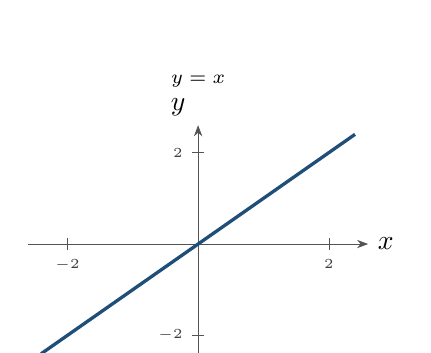
\begin{tikzpicture}
  \begin{axis}[fnaxis, xmin=-2.6, xmax=2.6, ymin=-2.6, ymax=2.6,
      xtick={-2,2}, ytick={-2,2}, title={$y=x$}]
    \addplot[domain=-2.4:2.4]{x};
  \end{axis}
\end{tikzpicture}\hfill
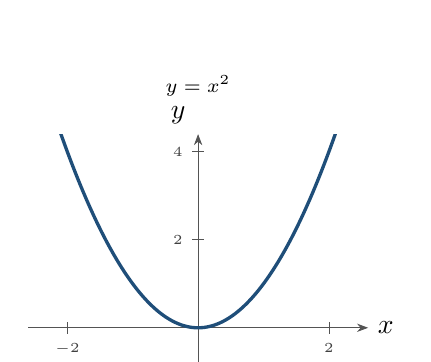
\begin{tikzpicture}
  \begin{axis}[fnaxis, xmin=-2.6, xmax=2.6, ymin=-1.0, ymax=4.4,
      xtick={-2,2}, ytick={2,4}, title={$y=x^{2}$}]
    \addplot[domain=-2.1:2.1]{x^2};
  \end{axis}
\end{tikzpicture}\hfill
\begin{tikzpicture}
  \begin{axis}[fnaxis, xmin=-2.6, xmax=2.6, ymin=-4.4, ymax=4.4,
      xtick={-2,2}, ytick={-4,4}, title={$y=x^{3}$}]
    \addplot[domain=-1.62:1.62]{x^3};
  \end{axis}
\end{tikzpicture}
\end{gallery}

\begin{gallery}
\begin{tikzpicture}
  \begin{axis}[fnaxis, xmin=-0.6, xmax=4.6, ymin=-0.8, ymax=2.6,
      xtick={2,4}, ytick={1,2}, title={$y=\sqrt{x}$}]
    \addplot[domain=0:4.4]{sqrt(x)};
  \end{axis}
\end{tikzpicture}\hfill
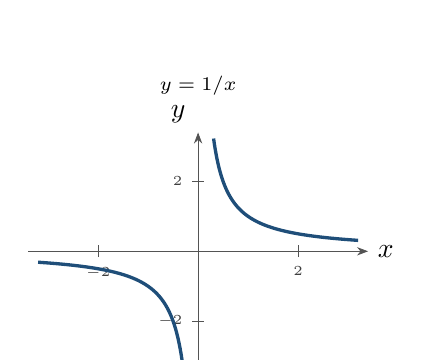
\begin{tikzpicture}
  \begin{axis}[fnaxis, xmin=-3.4, xmax=3.4, ymin=-3.4, ymax=3.4,
      xtick={-2,2}, ytick={-2,2}, title={$y=1/x$}]
    \addplot[domain=-3.2:-0.31]{1/x};
    \addplot[domain=0.31:3.2]{1/x};
  \end{axis}
\end{tikzpicture}\hfill
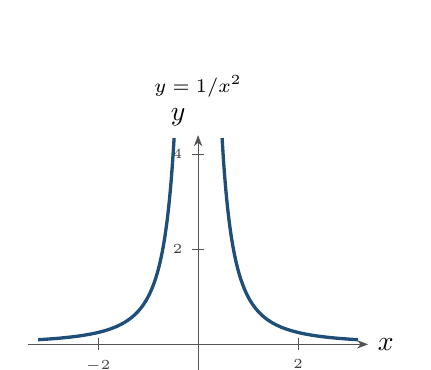
\begin{tikzpicture}
  \begin{axis}[fnaxis, xmin=-3.4, xmax=3.4, ymin=-0.6, ymax=4.4,
      xtick={-2,2}, ytick={2,4}, title={$y=1/x^{2}$}]
    \addplot[domain=-3.2:-0.48]{1/x^2};
    \addplot[domain=0.48:3.2]{1/x^2};
  \end{axis}
\end{tikzpicture}
\end{gallery}

\begin{rulebox}{Exponential, logarithm, absolute value}
$\mathrm{e}^{x}$ is positive everywhere, strictly increasing, and flattens
onto the asymptote $y=0$ as $x\to-\infty$; it passes through $(0,1)$.
$\ln x$ is its mirror image at the line $y=x$: defined only for $x>0$,
strictly increasing, passing through $(1,0)$, with the $y$-axis as a
vertical asymptote. A general exponential $a^{x}$ rises for $a>1$ and falls
for $0<a<1$, always through $(0,1)$; note $\bigl(\tfrac12\bigr)^{x}
=2^{-x}$, so the decreasing case is the increasing one reflected in the
$y$-axis. The absolute value $|x|$ is a V with its vertex at the origin.
\end{rulebox}

\begin{gallery}
\begin{tikzpicture}
  \begin{axis}[fnaxis, xmin=-3.4, xmax=2.4, ymin=-0.8, ymax=4.4,
      xtick={-2,2}, ytick={1,3}, title={$y=\mathrm{e}^{x}$}]
    \addplot[domain=-3.2:1.45]{exp(x)};
  \end{axis}
\end{tikzpicture}\hfill
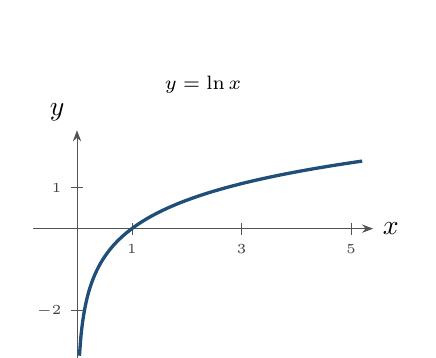
\begin{tikzpicture}
  \begin{axis}[fnaxis, xmin=-0.8, xmax=5.4, ymin=-3.4, ymax=2.4,
      xtick={1,3,5}, ytick={-2,1}, title={$y=\ln x$}]
    \addplot[domain=0.045:5.2]{ln(x)};
  \end{axis}
\end{tikzpicture}\hfill
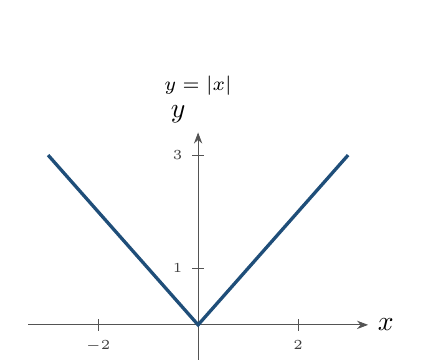
\begin{tikzpicture}
  \begin{axis}[fnaxis, xmin=-3.4, xmax=3.4, ymin=-0.8, ymax=3.4,
      xtick={-2,2}, ytick={1,3}, title={$y=|x|$}]
    \addplot[domain=-3:3]{abs(x)};
  \end{axis}
\end{tikzpicture}
\end{gallery}

\begin{rulebox}{What can be read off a formula without calculus}
\begin{itemize}[leftmargin=1.6em,itemsep=0.3ex]
  \item \textbf{$y$-intercept:} evaluate $f(0)$ (if $0\in D$).
  \item \textbf{Roots} \de{(Nullstellen)}: solve $f(x)=0$. For a product,
        set each factor to zero. A factor $(x-a)^{k}$ with $k$ odd makes
        the graph \emph{cross} the axis at $a$; with $k$ even it only
        \emph{touches} it.
  \item \textbf{Sign:} between consecutive roots and poles the sign cannot
        change. Pick one test point per interval; that fixes the whole
        picture.
  \item \textbf{Symmetry:} $f(-x)=f(x)$ gives mirror symmetry in the
        $y$-axis, $f(-x)=-f(x)$ point symmetry in the origin.
  \item \textbf{End behaviour of a polynomial:} only the leading term
        $a_{n}x^{n}$ matters as $x\to\pm\infty$. Even $n$: both ends go the
        same way (up if $a_{n}>0$). Odd $n$: the ends go opposite ways
        (down--left, up--right if $a_{n}>0$).
\end{itemize}
\end{rulebox}

\begin{rulebox}{Rational functions: poles and asymptotes}
Write $f(x)=\dfrac{p(x)}{q(x)}$ with $p,q$ polynomials and
\textbf{cancel common factors first}.
\begin{itemize}[leftmargin=1.6em,itemsep=0.3ex]
  \item A zero of $q$ that does \emph{not} cancel is a \textbf{pole}
        \de{(Polstelle)}: the vertical line $x=a$ is a
        \textbf{vertical asymptote}, and $|f|\to\infty$ there.
  \item A zero of $q$ that \emph{does} cancel is a \textbf{hole}: the graph
        is that of the reduced function, minus the single point $x=a$.
  \item \textbf{Horizontal asymptote}, by comparing degrees:
        $\deg p<\deg q\Rightarrow y=0$; \;$\deg p=\deg q\Rightarrow
        y=\dfrac{\text{leading coeff. of }p}{\text{leading coeff. of }q}$;
        \;$\deg p>\deg q\Rightarrow$ none.
  \item If $\deg p=\deg q+1$, polynomial division gives
        $f(x)=(\text{linear})+\dfrac{\text{remainder}}{q(x)}$, and the
        linear part is an \textbf{oblique asymptote}
        \de{(schiefe Asymptote)}, because the remainder term dies out.
\end{itemize}
\end{rulebox}

\begin{gallery}
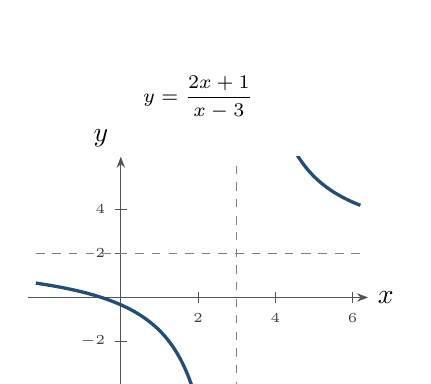
\begin{tikzpicture}
  \begin{axis}[fnaxis, xmin=-2.4, xmax=6.4, ymin=-4.4, ymax=6.4,
      xtick={2,4,6}, ytick={-2,2,4}, title={$y=\dfrac{2x+1}{x-3}$}]
    \addplot[domain=-2.2:2.55]{(2*x+1)/(x-3)};
    \addplot[domain=3.42:6.2]{(2*x+1)/(x-3)};
    \addplot[gray, dashed, thin, forget plot, samples=2, domain=-2.2:6.2]{2};
    \addplot[gray, dashed, thin, forget plot, samples=2] coordinates {(3,-4.2)(3,6.2)};
  \end{axis}
\end{tikzpicture}\hfill
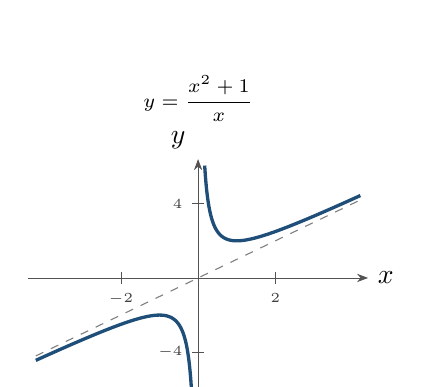
\begin{tikzpicture}
  \begin{axis}[fnaxis, xmin=-4.4, xmax=4.4, ymin=-6.4, ymax=6.4,
      xtick={-2,2}, ytick={-4,4}, title={$y=\dfrac{x^{2}+1}{x}$}]
    \addplot[domain=-4.2:-0.17]{(x^2+1)/x};
    \addplot[domain=0.17:4.2]{(x^2+1)/x};
    \addplot[gray, dashed, thin, forget plot, samples=2, domain=-4.2:4.2]{x};
  \end{axis}
\end{tikzpicture}\hfill
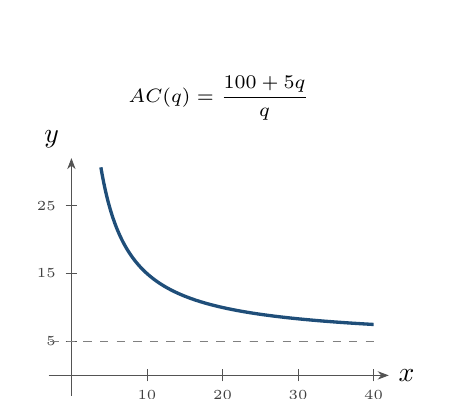
\begin{tikzpicture}
  \begin{axis}[fnaxis, xmin=-3, xmax=42, ymin=-3, ymax=32,
      xtick={10,20,30,40}, ytick={5,15,25},
      title={$AC(q)=\dfrac{100+5q}{q}$}]
    \addplot[domain=3.9:40]{(100+5*x)/x};
    \addplot[gray, dashed, thin, forget plot, samples=2, domain=-2.8:40]{5};
  \end{axis}
\end{tikzpicture}
\gcap{Horizontal asymptote $y=2$ and pole $x=3$ \quad\textbullet\quad
oblique asymptote $y=x$ \quad\textbullet\quad average cost falling towards
the asymptote $AC=5$.}
\end{gallery}

\begin{rulebox}{Curves given by an equation in two variables}
Not every curve is a graph $y=f(x)$. The standard ones:
\begin{itemize}[leftmargin=1.6em,itemsep=0.3ex]
  \item \textbf{Line:} $ax+by=c$. Sketch it from the two intercepts
        $x=c/a$ and $y=c/b$; solved for $y$ the slope is $-a/b$. This is
        the budget line $p_{x}x+p_{y}y=M$, with slope $-p_{x}/p_{y}$.
  \item \textbf{Circle:} $(x-x_{0})^{2}+(y-y_{0})^{2}=r^{2}$, centre
        $(x_{0},y_{0})$, radius $r$. A general
        $x^{2}+y^{2}+Dx+Ey+F=0$ is brought to this form by
        \textbf{completing the square} in $x$ and in $y$.
  \item \textbf{Ellipse:} $\dfrac{x^{2}}{a^{2}}+\dfrac{y^{2}}{b^{2}}=1$,
        crossing the axes at $(\pm a,0)$ and $(0,\pm b)$.
  \item \textbf{Hyperbola:} $xy=c$ with $c>0$ lies in the first and third
        quadrant with both axes as asymptotes. Solved for $y$ it is
        $y=c/x$. Every Cobb--Douglas isoquant $K^{\alpha}L^{\beta}=\bar Q$
        and every indifference curve $xy=\bar U$ has this shape.
\end{itemize}
To sketch, either solve for $y$, remembering that a square root splits the
curve into \textbf{two branches} $y=\pm\sqrt{\cdots}$, or read off centre,
radius and intercepts directly.
\end{rulebox}

\section{Practice Problems}

For each polynomial in problems 1--8, give the roots (with multiplicity
where it matters), the $y$-intercept, the symmetry, and the end behaviour
as $x\to\pm\infty$.

\begin{problems}
  \item $f(x)=x^{3}-4x$
  \item $f(x)=x^{4}-5x^{2}+4$
  \item $f(x)=-2x^{3}+6x$
  \item $f(x)=(x-1)^{2}(x+3)$
  \item $f(x)=x^{2}-6x+8$
  \item $f(x)=-x^{2}+4x-4$
  \item $f(x)=x^{5}-x$
  \item A polynomial satisfies $f(x)\to-\infty$ both as $x\to+\infty$ and
        as $x\to-\infty$. What does that say about its degree and its
        leading coefficient?
\end{problems}

In problems 9--20, give all vertical asymptotes, holes, and horizontal or
oblique asymptotes.

\begin{problems}[resume]
  \item $f(x)=\dfrac{1}{x-3}$
  \item $f(x)=\dfrac{2x+1}{x-3}$
  \item $f(x)=\dfrac{x^{2}-1}{x-1}$
  \item $f(x)=\dfrac{3x}{x^{2}-4}$
  \item $f(x)=\dfrac{x^{2}+1}{x}$
  \item $f(x)=\dfrac{x^{2}-4}{x^{2}-9}$
  \item $f(x)=\dfrac{x^{2}+3x+2}{x+1}$
  \item $f(x)=\dfrac{x^{2}-x-6}{x-3}$
  \item $f(x)=\dfrac{2x^{2}+3}{x-1}$
  \item $f(x)=\dfrac{5}{x^{2}+1}$
  \item $AC(q)=\dfrac{100+5q}{q}$ \;(average cost, $q>0$)
  \item $f(x)=\dfrac{x+3}{x^{2}+x-6}$
\end{problems}

\begin{problems}[resume]
  \item For $y=2^{x}$: give the $y$-intercept, the asymptote, the
        monotonicity and the range.
  \item Explain why the graph of $y=\bigl(\tfrac12\bigr)^{x}$ is the graph
        of $y=2^{x}$ reflected in the $y$-axis.
  \item For $y=\ln x$: give the $x$-intercept, the asymptote, the domain
        and the range.
  \item Sketch $y=\mathrm{e}^{-x}$ and state its asymptote and range.
  \item Both $\ln x$ and $\log_{10}x$ pass through $(1,0)$ and rise. What
        exactly distinguishes their graphs?
  \item The adjustment path $y=1-\mathrm{e}^{-x}$, $x\ge0$, is used for
        saturation effects. Give $y(0)$, the asymptote, and say in words
        what the curve does.
\end{problems}

\begin{problems}[resume]
  \item Match each graph (A)--(F) below to one of the formulas
        $\;\ln x$, \;$|x|$, \;$\sqrt{x}$, \;$x^{3}-x$,
        \;$\mathrm{e}^{-x}$, \;$1/x^{2}$.
\end{problems}

\begin{gallery}
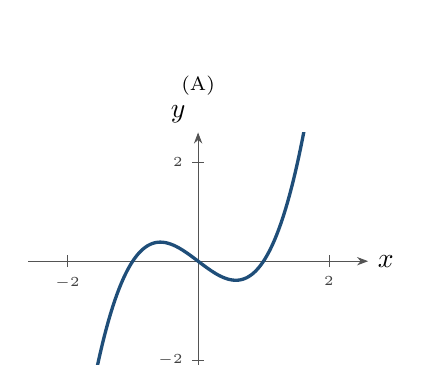
\begin{tikzpicture}
  \begin{axis}[fnaxis, xmin=-2.6, xmax=2.6, ymin=-2.2, ymax=2.6,
      xtick={-2,2}, ytick={-2,2}, title={(A)}]
    \addplot[domain=-1.85:1.85]{x^3-x};
  \end{axis}
\end{tikzpicture}\hfill
\begin{tikzpicture}
  \begin{axis}[fnaxis, xmin=-0.7, xmax=4.6, ymin=-0.8, ymax=2.6,
      xtick={2,4}, ytick={1,2}, title={(B)}]
    \addplot[domain=0:4.4]{sqrt(x)};
  \end{axis}
\end{tikzpicture}\hfill
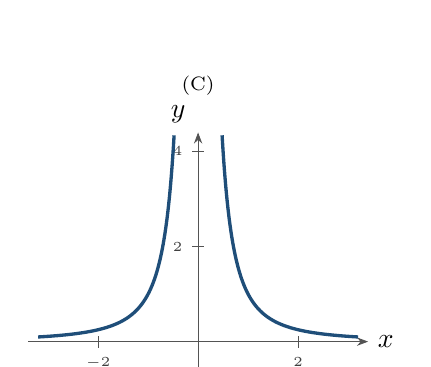
\begin{tikzpicture}
  \begin{axis}[fnaxis, xmin=-3.4, xmax=3.4, ymin=-0.6, ymax=4.4,
      xtick={-2,2}, ytick={2,4}, title={(C)}]
    \addplot[domain=-3.2:-0.48]{1/x^2};
    \addplot[domain=0.48:3.2]{1/x^2};
  \end{axis}
\end{tikzpicture}
\end{gallery}

\begin{gallery}
\begin{tikzpicture}
  \begin{axis}[fnaxis, xmin=-2.4, xmax=3.4, ymin=-0.8, ymax=4.4,
      xtick={-2,2}, ytick={1,3}, title={(D)}]
    \addplot[domain=-1.45:3.2]{exp(-x)};
  \end{axis}
\end{tikzpicture}\hfill
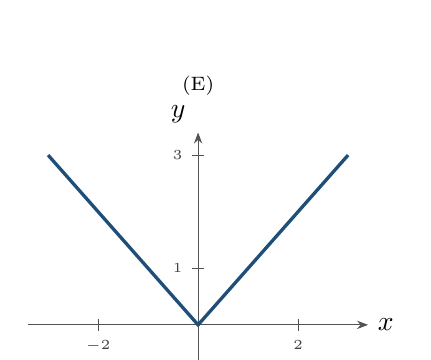
\begin{tikzpicture}
  \begin{axis}[fnaxis, xmin=-3.4, xmax=3.4, ymin=-0.8, ymax=3.4,
      xtick={-2,2}, ytick={1,3}, title={(E)}]
    \addplot[domain=-3:3]{abs(x)};
  \end{axis}
\end{tikzpicture}\hfill
\begin{tikzpicture}
  \begin{axis}[fnaxis, xmin=-0.8, xmax=5.4, ymin=-3.4, ymax=2.4,
      xtick={1,3,5}, ytick={-2,1}, title={(F)}]
    \addplot[domain=0.045:5.2]{ln(x)};
  \end{axis}
\end{tikzpicture}
\end{gallery}

\begin{problems}[resume]
  \item Sketch $f(x)=x^{2}-4x+3$: give the vertex, both intercepts and the
        direction of opening.
  \item Sketch $f(x)=\dfrac{x+1}{x-1}$: give both asymptotes and both
        intercepts.
  \item Sketch $f(x)=\sqrt{x+4}$: give the domain, the range and the
        starting point of the curve.
  \item Sketch $f(x)=|x|-2$: give the vertex and the roots.
  \item Sketch $f(x)=x^{3}-3x^{2}$: give the roots with multiplicity and
        the end behaviour.
  \item Classify as even, odd, or neither: (a) $x^{4}+2$, \;(b) $x^{3}+x$,
        \;(c) $1/x^{2}$, \;(d) $\mathrm{e}^{x}$.
  \item Which of these have a horizontal asymptote, and what is it?
        (a) $\dfrac{3x+1}{x-2}$, \;(b) $\dfrac{x^{2}}{x+1}$,
        \;(c) $\mathrm{e}^{-x}$ as $x\to+\infty$, \;(d) $\ln x$.
  \item On which intervals is $f(x)=\dfrac{(x-1)(x+2)}{x-3}$ positive?
  \item Describe the graph of $f(x)=\sqrt{x^{2}-1}$: domain, symmetry,
        range, and the two points where it meets the $x$-axis.
\end{problems}

In problems 37--45, identify the curve, and sketch it.

\begin{problems}[resume]
  \item $x^{2}+y^{2}=16$. Also solve for $y$ and give the two branches with
        their domains.
  \item $(x-2)^{2}+(y+1)^{2}=9$. Give centre and radius.
  \item $\dfrac{x^{2}}{9}+\dfrac{y^{2}}{4}=1$. Give the four axis
        intercepts.
  \item $xy=6$. Solve for $y$; in which quadrants does the curve lie?
  \item $y^{2}=x$. Is $y$ a function of $x$? Is $x$ a function of $y$?
  \item $2x+3y=12$. Give both intercepts and the slope.
  \item $x^{2}+y^{2}-4x+6y+9=0$. Complete the square; give centre and
        radius.
  \item The isoquant $K^{0.5}L^{0.5}=10$. Solve for $L$ and describe the
        shape for $K>0$.
  \item The budget line $4x+2y=40$ and the indifference curve $xy=50$.
        Give the slope of the budget line and $y$ as a function of $x$ on
        the indifference curve.
\end{problems}

\section{Solutions}

\begin{solutions}
  \item $x^{3}-4x=x(x^{2}-4)=x(x-2)(x+2)$: roots $-2,0,2$, all simple, all
        crossings; $f(0)=0$; odd (only odd powers); degree $3$ with
        positive leading coefficient, so $f\to-\infty$ as $x\to-\infty$ and
        $f\to+\infty$ as $x\to+\infty$.
  \item $x^{4}-5x^{2}+4=(x^{2}-1)(x^{2}-4)$: roots $\pm1,\pm2$;
        $f(0)=4$; even; degree $4$, positive leading coefficient, so both
        ends go to $+\infty$ (a W-shape).
  \item $-2x^{3}+6x=-2x(x^{2}-3)$: roots $0,\pm\sqrt3$; $f(0)=0$; odd;
        degree $3$ with \emph{negative} leading coefficient, so
        $f\to+\infty$ as $x\to-\infty$ and $f\to-\infty$ as $x\to+\infty$.
  \item Roots $x=1$ (double, the graph touches and turns back) and $x=-3$
        (simple, a crossing); $f(0)=(-1)^{2}\cdot3=3$; neither even nor
        odd; degree $3$, leading coefficient $+1$: down on the left, up on
        the right.
  \item $(x-2)(x-4)$: roots $2$ and $4$; $f(0)=8$; vertex at
        $x=3$, $f(3)=-1$; neither even nor odd; parabola opening upwards,
        both ends $+\infty$.
  \item $-(x-2)^{2}$: a double root at $x=2$ (the vertex touches the axis);
        $f(0)=-4$; opens downwards, both ends $-\infty$.
  \item $x^{5}-x=x(x^{4}-1)=x(x^{2}-1)(x^{2}+1)$: roots $-1,0,1$;
        $f(0)=0$; odd; degree $5$, positive leading coefficient: down on
        the left, up on the right.
  \item Both ends behave alike, so the degree is \textbf{even}; both go
        \emph{down}, so the leading coefficient is \textbf{negative}.
  \item Vertical asymptote $x=3$; $\deg p=0<1=\deg q$, so the horizontal
        asymptote is $y=0$. No holes.
  \item Vertical asymptote $x=3$; equal degrees, so
        $y=\tfrac{2}{1}=2$ is the horizontal asymptote.
  \item $\dfrac{(x-1)(x+1)}{x-1}=x+1$ for $x\neq1$: no pole but a
        \textbf{hole} at $(1,2)$. The graph is the line $y=x+1$ with that
        one point punched out; no horizontal asymptote.
  \item $x^{2}-4=(x-2)(x+2)$: poles at $x=\pm2$; $\deg p=1<2=\deg q$, so
        $y=0$.
  \item Pole at $x=0$. Degrees differ by one, so divide:
        $\dfrac{x^{2}+1}{x}=x+\dfrac{1}{x}$, giving the oblique asymptote
        $y=x$.
  \item Poles at $x=\pm3$; equal degrees with leading coefficients $1$ and
        $1$, so the horizontal asymptote is $y=1$.
  \item $\dfrac{(x+1)(x+2)}{x+1}=x+2$ for $x\neq-1$: a hole at $(-1,1)$,
        no pole, no horizontal asymptote.
  \item $\dfrac{(x-3)(x+2)}{x-3}=x+2$ for $x\neq3$: a hole at $(3,5)$.
  \item Pole at $x=1$. Division: $2x^{2}+3=(x-1)(2x+2)+5$, so
        $f(x)=2x+2+\dfrac{5}{x-1}$ and the oblique asymptote is $y=2x+2$.
  \item $x^{2}+1$ never vanishes: no poles at all. $\deg p=0<2$, so
        $y=0$; the graph is a bell-shaped hump with maximum $5$ at $x=0$,
        even.
  \item $AC(q)=\dfrac{100}{q}+5$: pole at $q=0$ and horizontal asymptote
        $AC=5$. Average cost falls towards the marginal cost $5$ as the
        fixed cost $100$ is spread over more units.
  \item $x^{2}+x-6=(x+3)(x-2)$, so
        $f(x)=\dfrac{x+3}{(x+3)(x-2)}=\dfrac{1}{x-2}$ for $x\neq-3$:
        a hole at $\bigl(-3,-\tfrac15\bigr)$, a pole at $x=2$, and the
        horizontal asymptote $y=0$.
  \item $y$-intercept $2^{0}=1$; asymptote $y=0$ (approached as
        $x\to-\infty$); strictly increasing; range $(0,\infty)$.
  \item Because $\bigl(\tfrac12\bigr)^{x}=(2^{-1})^{x}=2^{-x}$: the
        argument $x$ has been replaced by $-x$, and replacing $x$ by $-x$
        mirrors any graph in the $y$-axis.
  \item $x$-intercept $(1,0)$; the $y$-axis $x=0$ is a vertical asymptote
        (as $x\to0^{+}$, $\ln x\to-\infty$); $D=(0,\infty)$, $W=\R$.
  \item The decreasing exponential: it falls from $+\infty$ through
        $(0,1)$ towards the asymptote $y=0$ as $x\to+\infty$;
        $W=(0,\infty)$. It is $\mathrm{e}^{x}$ mirrored in the $y$-axis.
  \item Only the vertical scale: $\log_{10}x=\dfrac{\ln x}{\ln 10}$, so the
        common logarithm is the natural one compressed by the constant
        factor $\ln 10\approx2.303$. Same domain, same asymptote, same
        intercept, same shape.
  \item $y(0)=1-1=0$; as $x\to\infty$, $\mathrm{e}^{-x}\to0$, so the
        asymptote is $y=1$. The curve starts at the origin, rises steeply
        at first and then ever more slowly, approaching the saturation
        level $1$ without ever reaching it.
  \item (A) $x^{3}-x$ \;(odd, three roots); \;(B) $\sqrt{x}$;
        \;(C) $1/x^{2}$ \;(even, positive, pole at $0$);
        \;(D) $\mathrm{e}^{-x}$; \;(E) $|x|$; \;(F) $\ln x$.
  \item $x^{2}-4x+3=(x-1)(x-3)=(x-2)^{2}-1$: opens upwards, vertex
        $(2,-1)$, roots $1$ and $3$, $y$-intercept $3$.
  \item $\dfrac{x+1}{x-1}$: pole $x=1$, horizontal asymptote $y=1$ (equal
        degrees); root $x=-1$; $y$-intercept $f(0)=-1$. Two branches, one
        in each half-plane of the pole.
  \item $D=[-4,\infty)$, $W=[0,\infty)$; the curve starts at $(-4,0)$ and
        rises, ever more slowly: the $\sqrt{\;}$ shape moved four units to
        the left.
  \item A V with vertex $(0,-2)$; roots where $|x|=2$, i.e. $x=\pm2$;
        $y$-intercept $-2$.
  \item $x^{3}-3x^{2}=x^{2}(x-3)$: a double root at $x=0$ (touch) and a
        simple root at $x=3$ (crossing); degree $3$, positive leading
        coefficient: down on the left, up on the right.
  \item (a) even; (b) odd; (c) even, since $1/(-x)^{2}=1/x^{2}$;
        (d) neither.
  \item (a) yes, $y=3$ (equal degrees); (b) no: the numerator degree
        exceeds the denominator degree by one, so there is an oblique
        asymptote $y=x-1$ instead; (c) yes, $y=0$; (d) no: $\ln x$ grows
        without bound, however slowly.
  \item Critical points $-2,1,3$. Test one point per interval:
        $x=-3$ gives $\frac{(-4)(-1)}{-6}<0$; $x=0$ gives
        $\frac{(-1)(2)}{-3}>0$; $x=2$ gives $\frac{(1)(4)}{-1}<0$;
        $x=4$ gives $\frac{(3)(6)}{1}>0$. Hence $f>0$ on
        $(-2,1)\cup(3,\infty)$.
  \item $D=(-\infty,-1]\cup[1,\infty)$ (from $x^{2}-1\ge0$); even, so
        symmetric about the $y$-axis; $W=[0,\infty)$; it meets the axis at
        $(-1,0)$ and $(1,0)$ and rises from there, approaching the lines
        $y=\pm x$ from below for large $|x|$.
  \item Circle, centre $(0,0)$, radius $4$. Solving:
        $y=\pm\sqrt{16-x^{2}}$, two branches, each with domain $[-4,4]$;
        the plus sign is the upper semicircle, the minus sign the lower.
  \item Circle with centre $(2,-1)$ and radius $3$.
  \item Ellipse with $a=3$ and $b=2$: it crosses the axes at
        $(\pm3,0)$ and $(0,\pm2)$.
  \item $y=6/x$, a hyperbola with both axes as asymptotes. Since the
        product is positive, $x$ and $y$ share a sign: the curve lies in
        the first and third quadrants.
  \item A parabola opening to the right. $y$ is \emph{not} a function of
        $x$: the line $x=4$ meets the curve at $y=\pm2$. But $x=y^{2}$
        \emph{is} a function of $y$.
  \item Intercepts $(6,0)$ and $(0,4)$; solved for $y$,
        $y=4-\tfrac23 x$, so the slope is $-\tfrac23$.
  \item $(x^{2}-4x+4)+(y^{2}+6y+9)=-9+4+9$, i.e.
        $(x-2)^{2}+(y+3)^{2}=4$: centre $(2,-3)$, radius $2$.
  \item $K^{0.5}L^{0.5}=10\Rightarrow (KL)^{0.5}=10\Rightarrow KL=100
        \Rightarrow L=\dfrac{100}{K}$. A hyperbola in the first quadrant,
        falling and convex, with both axes as asymptotes: the familiar
        isoquant, along which more capital buys ever less labour saving.
  \item Budget line: $y=20-2x$, slope $-2$ (the price ratio
        $-p_{x}/p_{y}=-4/2$), intercepts $(10,0)$ and $(0,20)$.
        Indifference curve: $y=50/x$, a hyperbola in the first quadrant.
\end{solutions}

\section{Additional Problems}

\begin{problems}
  \item Asymptotes of $f(x)=\dfrac{4x-1}{2x+6}$.
  \item Asymptotes and holes of $f(x)=\dfrac{x^{2}-9}{x+3}$.
  \item Asymptotes and symmetry of $f(x)=\dfrac{x^{3}}{x^{2}-1}$.
  \item Asymptotes and holes of $f(x)=\dfrac{x^{2}-2x}{x^{2}-4}$.
  \item Asymptotes of $f(x)=\dfrac{6}{x^{2}-x-2}$.
  \item Asymptotes of $f(x)=\dfrac{x-4}{x^{2}+4}$.
  \item Roots, symmetry and end behaviour of $f(x)=x^{4}-4x^{2}$.
  \item Roots, sign and end behaviour of $f(x)=(x+2)(x-1)(x-3)$.
  \item Symmetry and asymptote of $f(x)=\dfrac{x}{x^{2}+1}$.
  \item Where do $y=3^{x}$ and $y=3^{-x}$ intersect, and what asymptote do
        they share?
  \item The graphs of $y=\mathrm{e}^{x}$ and $y=\ln x$ are mirror images.
        In which line, and which points correspond to each other?
  \item Domain, range, symmetry and asymptotes of $y=1/x^{2}$.
  \item Domain, symmetry and shape of $y=\sqrt[3]{x}$.
  \item Vertex and roots of $y=|x-2|$.
  \item For the cost function $C(q)=q^{3}-6q^{2}+15q$, tabulate
        $C(0),C(1),\dots,C(5)$ and describe the shape of the curve.
  \item Tabulate $f(x)=x^{2}-2x-3$ for $x=-2,\dots,4$ and sketch it from
        the table; give vertex and roots.
  \item Identify $9x^{2}+4y^{2}=36$ and give its axis intercepts.
  \item Identify $x^{2}-y^{2}=9$ and solve it for $y$.
  \item What curve is $(x+1)^{2}+(y-2)^{2}=0$?
  \item Identify $x^{2}+y^{2}+2x-8=0$: centre and radius.
  \item Compare $y=\sqrt{9-x^{2}}$ with $x^{2}+y^{2}=9$: which is a
        function, and what are its domain and range?
  \item The isocost line $5K+2L=100$: give both intercepts and $L$ as a
        function of $K$.
  \item For the indifference curve $xy=36$, tabulate $y$ at
        $x=1,2,3,4,6,9,12$ and describe the shape.
  \item The demand curve $p=100/q$ has the property that revenue $pq$ is
        constant. Give that constant, the asymptotes, and the economic
        reading of each.
  \item A curve passes through the origin, rises throughout, is concave,
        and flattens onto the horizontal line $y=4$. Which of
        $y=4-\mathrm{e}^{-x}$, \;$y=4(1-\mathrm{e}^{-x})$,
        \;$y=4\mathrm{e}^{-x}$ fits, and why do the other two fail?
\end{problems}

\section{Additional Solutions}

\begin{solutions}
  \item Pole where $2x+6=0$, i.e. $x=-3$; equal degrees, so the horizontal
        asymptote is $y=\tfrac42=2$.
  \item $\dfrac{(x-3)(x+3)}{x+3}=x-3$ for $x\neq-3$: a hole at
        $(-3,-6)$, no pole, no horizontal asymptote (the graph is a line).
  \item Poles at $x=\pm1$. Division: $x^{3}=x(x^{2}-1)+x$, so
        $f(x)=x+\dfrac{x}{x^{2}-1}$ and the oblique asymptote is $y=x$.
        Odd: numerator odd, denominator even.
  \item $\dfrac{x(x-2)}{(x-2)(x+2)}=\dfrac{x}{x+2}$ for $x\neq2$: a hole at
        $\bigl(2,\tfrac12\bigr)$, a pole at $x=-2$, horizontal asymptote
        $y=1$.
  \item $x^{2}-x-2=(x-2)(x+1)$: poles at $x=2$ and $x=-1$; horizontal
        asymptote $y=0$.
  \item $x^{2}+4>0$ always: no poles. Numerator degree smaller, so $y=0$.
  \item $x^{4}-4x^{2}=x^{2}(x^{2}-4)=x^{2}(x-2)(x+2)$: double root at $0$
        (touch), simple roots at $\pm2$; even; degree $4$ with positive
        leading coefficient, so both ends rise to $+\infty$.
  \item Roots $-2,1,3$, all simple. Degree $3$, positive leading
        coefficient: down on the left, up on the right. Signs alternate
        between the roots: negative on $(-\infty,-2)$, positive on
        $(-2,1)$, negative on $(1,3)$, positive on $(3,\infty)$.
  \item Odd (odd numerator over even denominator); no poles since
        $x^{2}+1>0$; horizontal asymptote $y=0$ at both ends. The graph is
        a hump above the axis on the right and its mirror image below on
        the left.
  \item $3^{x}=3^{-x}\iff x=-x\iff x=0$: they meet at $(0,1)$. Both have
        the horizontal asymptote $y=0$, the first as $x\to-\infty$, the
        second as $x\to+\infty$; each is the other reflected in the
        $y$-axis.
  \item In the line $y=x$. The point $(a,\mathrm{e}^{a})$ on the
        exponential corresponds to $(\mathrm{e}^{a},a)$ on the logarithm;
        in particular $(0,1)\leftrightarrow(1,0)$ and
        $(1,\mathrm{e})\leftrightarrow(\mathrm{e},1)$. The two functions
        are inverse to each other.
  \item $D=\R\setminus\{0\}$, $W=(0,\infty)$; even, hence symmetric about
        the $y$-axis; vertical asymptote $x=0$ and horizontal asymptote
        $y=0$. Both branches lie above the axis.
  \item $D=\R$: an odd root accepts negative radicands. It is odd, since
        $\sqrt[3]{-x}=-\sqrt[3]{x}$, strictly increasing, steep near the
        origin and flattening out: the graph of $x^{3}$ mirrored in
        $y=x$.
  \item A V with vertex $(2,0)$; a single (double) root at $x=2$;
        $y$-intercept $|0-2|=2$.
  \item $C(0)=0$, $C(1)=10$, $C(2)=14$, $C(3)=18$, $C(4)=28$, $C(5)=50$.
        Increasing throughout; the increments $10,4,4,10,22$ first fall and
        then rise, so the curve is concave up to about $q=2$ and convex
        afterwards: the S-shaped total cost curve of the textbooks, with
        its inflection at $q=2$.
  \item $f(-2)=5$, $f(-1)=0$, $f(0)=-3$, $f(1)=-4$, $f(2)=-3$, $f(3)=0$,
        $f(4)=5$. The table is symmetric about $x=1$: an upward parabola
        with vertex $(1,-4)$ and roots $-1$ and $3$.
  \item Divide by $36$: $\dfrac{x^{2}}{4}+\dfrac{y^{2}}{9}=1$, an ellipse
        with $a=2$, $b=3$, crossing the axes at $(\pm2,0)$ and
        $(0,\pm3)$.
  \item A hyperbola opening left and right. Solved for $y$:
        $y=\pm\sqrt{x^{2}-9}$, defined for $|x|\ge3$, two branches.
  \item A sum of two squares is zero only if both vanish: the ``curve'' is
        the single point $(-1,2)$.
  \item $(x+1)^{2}-1+y^{2}=8$, so $(x+1)^{2}+y^{2}=9$: a circle with centre
        $(-1,0)$ and radius $3$.
  \item $y=\sqrt{9-x^{2}}$ is a function, the upper semicircle, with
        $D=[-3,3]$ and $W=[0,3]$. The full equation $x^{2}+y^{2}=9$ is not
        a function of $x$: it also contains the lower half.
  \item Intercepts $(20,0)$ on the $K$-axis and $(0,50)$ on the $L$-axis;
        $L=50-2.5K$, a falling line with slope $-2.5$, the ratio of the
        input prices.
  \item $y=36/x$: $36,18,12,9,6,4,3$. A falling, convex hyperbola branch in
        the first quadrant, approaching both axes without touching them:
        halving $x$ doubles $y$.
  \item $pq=100$. The asymptotes are $p=0$ and $q=0$: as the quantity
        grows, the price falls towards zero without reaching it, and no
        finite price clears an arbitrarily small quantity. Revenue stays at
        $100$ everywhere, which is what unit elasticity means.
  \item $y=4(1-\mathrm{e}^{-x})$. It gives $y(0)=0$ and rises to the
        asymptote $4$. \;$y=4-\mathrm{e}^{-x}$ has the right asymptote but
        starts at $y(0)=3$, not at the origin; \;$y=4\mathrm{e}^{-x}$ falls
        from $4$ towards $0$ instead of rising.
\end{solutions}

\chapter{Partial Fractions}

Decompose each rational expression. Problems 2 and 3 are \emph{improper}
(numerator degree $\ge$ denominator degree): perform polynomial division
first.

\section{Core Rules}

\begin{rulebox}{What the method does, and why}
A partial fraction decomposition rewrites one complicated fraction as a sum
of simple ones:
\[
  \frac{7x+1}{(x+2)(x-3)}=\frac{A}{x+2}+\frac{B}{x-3} .
\]
It is the reverse of putting fractions over a common denominator. The point
is that each piece on the right is something you can integrate, invert, or
sum, while the left side is not.
\end{rulebox}

\begin{rulebox}{Step 0, which must not be skipped: make it proper}
The method applies only when $\deg(\text{numerator})<\deg(\text{denominator})$.
If not, \textbf{divide first}:
\[
  \frac{x^{2}}{(x-1)(x-2)}
  =\frac{x^{2}}{x^{2}-3x+2}
  =1+\frac{3x-2}{x^{2}-3x+2} ,
\]
and decompose only the remainder. An improper fraction fed straight into the
ansatz produces an unsolvable or inconsistent system.
\end{rulebox}

\begin{rulebox}{Choosing the ansatz}
Factor the denominator completely, then contribute one term per factor:
\begin{itemize}[leftmargin=1.6em,itemsep=0.3ex]
  \item \textbf{Distinct linear factor} $(x-a)$: one term $\dfrac{A}{x-a}$.
  \item \textbf{Repeated linear factor} $(x-a)^{k}$: \textbf{all} $k$ terms,
        \[
          \frac{A_{1}}{x-a}+\frac{A_{2}}{(x-a)^{2}}+\cdots+\frac{A_{k}}{(x-a)^{k}} .
        \]
  \item \textbf{Irreducible quadratic} $(x^{2}+px+q)$ with $p^{2}<4q$:
        a \emph{linear} numerator, $\dfrac{Bx+C}{x^{2}+px+q}$.
\end{itemize}
The numerator always has degree one less than its denominator factor.
\end{rulebox}

\begin{rulebox}{Finding the constants: two techniques}
Multiply through by the full denominator to get a polynomial identity, then
either
\begin{itemize}[leftmargin=1.6em,itemsep=0.3ex]
  \item \textbf{substitute the roots} (the ``cover-up'' method) --- each root
        of a linear factor eliminates every term but one, giving a constant
        immediately; or
  \item \textbf{compare coefficients} of like powers, giving a small linear
        system.
\end{itemize}
Roots are faster and handle the simple constants; coefficient comparison
supplies the ones the roots cannot reach, which is exactly the situation with
a repeated factor.
\end{rulebox}

\section{Worked Examples}

\begin{worked}{(a) Decompose $\dfrac{x^{2}-5}{x(x+1)^{2}}$}
\wstep{Step 1. Check properness, then write the ansatz.}
The numerator has degree $2$, the denominator degree $3$: proper, so no
division is needed. The factor $(x+1)$ is repeated, so it contributes
\emph{two} terms:
\[
  \frac{x^{2}-5}{x(x+1)^{2}}
  =\frac{A}{x}+\frac{B}{x+1}+\frac{C}{(x+1)^{2}} .
\]
\wtrap{Writing only $\dfrac{A}{x}+\dfrac{C}{(x+1)^{2}}$ is the classic error.
Two unknowns cannot match three coefficients, and the resulting system will
be inconsistent --- which at least tells you something is wrong. A repeated
factor of multiplicity $k$ needs all $k$ powers.}

\wstep{Step 2. Clear the denominators.}
Multiplying both sides by $x(x+1)^{2}$:
\[
  x^{2}-5=A(x+1)^{2}+Bx(x+1)+Cx .
\]
This is an identity: it holds for \emph{every} $x$, which is what licenses
the substitutions that follow.

\wstep{Step 3. Substitute the roots to find the easy constants.}
\[
  x=0:\quad -5=A(1)+0+0 \;\Longrightarrow\; A=-5 .
\]
\[
  x=-1:\quad 1-5=0+0+C(-1) \;\Longrightarrow\; -4=-C \;\Longrightarrow\; C=4 .
\]

\wstep{Step 4. Get $B$ by comparing coefficients.}
No substitution isolates $B$ --- that is characteristic of a repeated
factor. Compare the coefficient of $x^{2}$ on both sides:
\[
  1=A+B \;\Longrightarrow\; B=1-(-5)=6 .
\]
\wtrap{Only $A(x+1)^{2}$ and $Bx(x+1)$ produce an $x^{2}$; $Cx$ does not.
Expand mentally and take just the one coefficient you need rather than
multiplying everything out.}

\wstep{Step 5. Verify at a value not yet used.}
\[
  \frac{x^{2}-5}{x(x+1)^{2}}=\boxed{-\frac{5}{x}+\frac{6}{x+1}+\frac{4}{(x+1)^{2}}}
\]
Test $x=1$: the left side is $(1-5)/(1\cdot4)=-1$; the right side is
$-5+3+1=-1$. \checkmark\ One substitution catches nearly every arithmetic
slip, and it costs ten seconds.
\end{worked}

\begin{worked}{(b) The improper case: $\dfrac{x^{2}}{(x-1)(x-2)}$}
\wstep{Step 1. Compare degrees --- and stop.}
Numerator degree $2$, denominator degree $2$. The fraction is improper, so
the ansatz $\frac{A}{x-1}+\frac{B}{x-2}$ cannot possibly work: that sum
tends to $0$ as $x\to\infty$, while the left side tends to $1$.

\wstep{Step 2. Divide, by adding and subtracting rather than by long division.}
The denominator expands to $x^{2}-3x+2$, so
\[
  x^{2}=(x^{2}-3x+2)+(3x-2)
  \quad\Longrightarrow\quad
  \frac{x^{2}}{(x-1)(x-2)}=1+\frac{3x-2}{(x-1)(x-2)} .
\]

\wstep{Step 3. Decompose the proper remainder.}
\[
  \frac{3x-2}{(x-1)(x-2)}=\frac{A}{x-1}+\frac{B}{x-2}
  \quad\Longrightarrow\quad
  3x-2=A(x-2)+B(x-1).
\]
\[
  x=1:\ 1=A(-1)\Rightarrow A=-1 ;\qquad
  x=2:\ 4=B(1)\Rightarrow B=4 .
\]

\wstep{Step 4. Reassemble --- and do not lose the $1$.}
\[
  \frac{x^{2}}{(x-1)(x-2)}=\boxed{1-\frac{1}{x-1}+\frac{4}{x-2}}
\]
Check at $x=0$: left side $0$; right side $1-\frac{1}{-1}+\frac{4}{-2}
=1+1-2=0$. \checkmark
\wtrap{The polynomial part is part of the answer. Decomposing the remainder
and then reporting only the fractions loses a whole term --- and, in the
integration volume, loses the $x$ in the antiderivative.}
\end{worked}

\section{Practice Problems}

\begin{problems}
  \item $\displaystyle\frac{7x+1}{(x+2)(x-3)}$
  \item $\displaystyle\frac{x^{2}}{(x-1)(x-2)}$ (improper)
  \item $\displaystyle\frac{2x^{2}+5x-3}{(x+1)(x-2)}$ (improper)
  \item $\displaystyle\frac{4x-5}{x^{2}-3x+2}$
  \item $\displaystyle\frac{6x+1}{(x-1)(x+3)}$
  \item $\displaystyle\frac{x-5}{x(x-4)}$
  \item $\displaystyle\frac{1}{(x+4)(x+5)}$
  \item $\displaystyle\frac{x-4}{x^{2}+2x-8}$
  \item $\displaystyle\frac{1}{x^{2}-7x+12}$
  \item $\displaystyle\frac{2x^{2}+3}{x(x-1)(x+2)}$
  \item $\displaystyle\frac{x+2}{(x-1)^{2}}$
  \item $\displaystyle\frac{5x}{(x+2)^{2}}$
  \item $\displaystyle\frac{1}{x^{2}(x+1)}$
  \item $\displaystyle\frac{x^{2}-5}{x(x+1)^{2}}$
  \item $\displaystyle\frac{2x+3}{x^{2}+4x}$
  \item $\displaystyle\frac{1}{(x-1)(x^{2}-4)}$
  \item $\displaystyle\frac{5-x}{(x+3)(x-1)}$
  \item $\displaystyle\frac{4x-7}{(x-2)(x+1)(x+3)}$
  \item $\displaystyle\frac{1}{(s+a)(s+b)}$ ($a\neq b$, symbolic)
  \item $\displaystyle\frac{2K-1}{K(1-K)}$ (logistic-style)
  \item $\displaystyle\frac{3x^{2}+4x+1}{x^{3}}$
  \item $\displaystyle\frac{1}{(2s+1)(s-2)}$ (Laplace style)
  \item $\displaystyle\frac{6}{x^{2}-25}$
  \item $\displaystyle\frac{\mathrm{e}^{x}}{\mathrm{e}^{2x}-1}$
        (substitute $u=\mathrm{e}^{x}$ first)
  \item $\displaystyle\frac{3t+1}{t(t-1)(t-2)}$
  \item $\displaystyle\frac{x+4}{x^{3}+x^{2}}$
  \item $\displaystyle\frac{2y-3}{(y+1)^{2}}$
  \item $\displaystyle\frac{4x-5}{(x-3)^{2}}$
  \item $\displaystyle\frac{1}{(x+a)(x+b)}$ ($a\neq b$, symbolic)
  \item Telescoping: write $\displaystyle\frac{1}{(k-1)k}$ ($k\ge 2$) as a
        difference of two terms.
\end{problems}

\section{Solutions}

\begin{solutions}
  \item $\displaystyle\frac{13/5}{x+2}+\frac{22/5}{x-3}$
  \item $1-\displaystyle\frac{1}{x-1}+\frac{4}{x-2}$
  \item $2+\displaystyle\frac{2}{x+1}+\frac{5}{x-2}$
  \item $\displaystyle\frac{1}{x-1}+\frac{3}{x-2}$
  \item $\displaystyle\frac{7/4}{x-1}+\frac{17/4}{x+3}$
  \item $\displaystyle\frac{5/4}{x}-\frac{1/4}{x-4}$
  \item $\displaystyle\frac{1}{x+4}-\frac{1}{x+5}$
  \item $\displaystyle-\frac{1/3}{x-2}+\frac{4/3}{x+4}$
  \item $\displaystyle-\frac{1}{x-3}+\frac{1}{x-4}$
  \item $\displaystyle-\frac{3/2}{x}+\frac{5/3}{x-1}+\frac{11/6}{x+2}$
  \item $\displaystyle\frac{1}{x-1}+\frac{3}{(x-1)^{2}}$
  \item $\displaystyle\frac{5}{x+2}-\frac{10}{(x+2)^{2}}$
  \item $\displaystyle-\frac{1}{x}+\frac{1}{x^{2}}+\frac{1}{x+1}$
  \item $\displaystyle-\frac{5}{x}+\frac{6}{x+1}+\frac{4}{(x+1)^{2}}$
  \item $\displaystyle\frac{3/4}{x}+\frac{5/4}{x+4}$
  \item $\displaystyle-\frac{1/3}{x-1}+\frac{1/4}{x-2}+\frac{1/12}{x+2}$
  \item $\displaystyle-\frac{2}{x+3}+\frac{1}{x-1}$
  \item $\displaystyle\frac{1/15}{x-2}+\frac{11/6}{x+1}-\frac{19/10}{x+3}$
  \item $\displaystyle\frac{1}{b-a}\left(\frac{1}{s+a}-\frac{1}{s+b}\right)$
  \item $\displaystyle-\frac{1}{K}+\frac{1}{1-K}$
  \item $\displaystyle\frac{3}{x}+\frac{4}{x^{2}}+\frac{1}{x^{3}}$
  \item $\displaystyle-\frac{2/5}{2s+1}+\frac{1/5}{s-2}$
  \item $\displaystyle\frac{3/5}{x-5}-\frac{3/5}{x+5}$
  \item $\displaystyle\frac{1/2}{\mathrm{e}^{x}-1}+\frac{1/2}{\mathrm{e}^{x}+1}$
  \item $\displaystyle\frac{1/2}{t}-\frac{4}{t-1}+\frac{7/2}{t-2}$
  \item $\displaystyle-\frac{3}{x}+\frac{4}{x^{2}}+\frac{3}{x+1}$
  \item $\displaystyle\frac{2}{y+1}-\frac{5}{(y+1)^{2}}$
  \item $\displaystyle\frac{4}{x-3}+\frac{7}{(x-3)^{2}}$
  \item $\displaystyle\frac{1}{b-a}\left(\frac{1}{x+a}-\frac{1}{x+b}\right)$
  \item $\displaystyle\frac{1}{k-1}-\frac{1}{k}$
\end{solutions}

\chapter{Systems of Equations}

Solve each system for all variables.

\section{Practice Problems}

\begin{problems}
  \item \textbf{[Part A: Linear $2\times 2$ and economic models, 1--10.]}
        $3x+2y=16,\ x-y=-3$
  \item $4x+3y=17,\ 2x-y=1$
  \item $0.5x+0.3y=5.2,\ x+y=12$
  \item Equilibrium: $Q_{d}=80-2P,\ Q_{s}=-10+3P$
  \item IS-LM: $Y=600-200r,\ Y=400+200r$
  \item Break-even: $C=12+3Q,\ R=5Q$, find break-even $Q$.
  \item $2x+3y=6,\ 4x+6y=15$
  \item $x-y=4,\ 3x-3y=12$
  \item $5x-3y=1,\ 2x+y=7$
  \item Capital--labour: $L=2K,\ wL+rK=C$ with $w=3,\,r=4,\,C=50$
  \item \textbf{[Part B: Non-linear $2\times 2$, 11--15.]}
        $y=x^{2}-4,\ y=-x^{2}+4$
  \item $xy=18,\ x-y=3$
  \item $x^{2}+y^{2}=20,\ x=2y$
  \item $y=\mathrm{e}^{x},\ y=\mathrm{e}^{2-x}$
  \item $\sqrt{x}+y=4,\ y=x-2$ (check for extraneous roots)
  \item \textbf{[Part C: Lagrangian-style systems, 16--22.]}
        Cobb--Douglas: $\dfrac{\alpha}{x}=\lambda p_{x},\
        \dfrac{1-\alpha}{y}=\lambda p_{y},\ p_{x}x+p_{y}y=I$, solve
        for $x,y$.
  \item CES capital--labour ratio: $\alpha K^{\rho-1}=\lambda r,\
        (1-\alpha)L^{\rho-1}=\lambda w$, find $K/L$.
  \item $2x=\lambda,\ \lambda=4y,\ 3x+y=14$
  \item $\lambda y=6,\ \lambda x=4,\ xy=24$ ($\lambda>0$)
  \item $4=\lambda K,\ 1=\lambda L,\ K+L=10$
  \item Quasi-linear: $1=\lambda p_{x},\ \dfrac{1}{y}=\lambda p_{y},\
        p_{x}x+p_{y}y=I$, solve for $x,y$.
  \item Simplex: $\alpha x^{\alpha-1}y^{1-\alpha}=\lambda,\
        (1-\alpha)x^{\alpha}y^{-\alpha}=\lambda,\ x+y=1$
  \item \textbf{[Part D: Linear $3\times 3$, 23--30.]}
        $x+y-z=2,\ 2x-y+z=4,\ -x+y+2z=1$
  \item $x+y+z=12,\ 2x+3y-z=13,\ x-y+2z=9$
  \item $x+y+z=2,\ 2x-y-z=1,\ x+2y-z=-3$
  \item $x+y+z=60,\ y=2x,\ z=x+y$
  \item $x+2y+3z=11,\ 4x+y+2z=17,\ 3x+5y+z=16$
  \item $x-y=1,\ y-z=1,\ x+y+z=6$
  \item $x+y+z=3,\ x+2y-z=1,\ -x+y+2z=0$
  \item $2x+y-z=2,\ x-2y+z=0,\ 3x+y+2z=6$
\end{problems}

\section{Solutions}

\begin{solutions}
  \item $x=2,\ y=5$
  \item $x=2,\ y=3$
  \item $x=8,\ y=4$
  \item $P=18,\ Q=44$
  \item $r=\tfrac12,\ Y=500$
  \item $Q=6$
  \item No solution (parallel lines).
  \item Infinitely many solutions (same line).
  \item $x=2,\ y=3$
  \item $K=5,\ L=10$
  \item $(2,0)$ and $(-2,0)$
  \item $(6,3)$ and $(-3,-6)$
  \item $(4,2)$ and $(-4,-2)$
  \item $(1,\mathrm{e})$
  \item $(4,2)$ only; $(9,7)$ is extraneous because
        $\sqrt{9}=3\neq 6-9$.
  \item $x=\dfrac{\alpha I}{p_{x}},\ y=\dfrac{(1-\alpha)I}{p_{y}},\
        \lambda=\dfrac{1}{I}$
  \item $\dfrac{K}{L}=\left(\dfrac{(1-\alpha)r}{\alpha w}\right)^{1/(\rho-1)}$
  \item $x=4,\ y=2,\ \lambda=8$
  \item $\lambda=1,\ x=4,\ y=6$
  \item $\lambda=\tfrac12,\ K=8,\ L=2$
  \item $\lambda=\dfrac{1}{p_{x}},\ y=\dfrac{p_{x}}{p_{y}},\
        x=\dfrac{I}{p_{x}}-1$
  \item $x=\alpha,\ y=1-\alpha$
  \item $(2,1,1)$
  \item $(3,4,5)$
  \item $(1,-1,2)$
  \item $x=10,\ y=20,\ z=30$
  \item $(3,1,2)$
  \item $(3,2,1)$
  \item $(2,0,1)$
  \item $(1,1,1)$
\end{solutions}

\chapter{Summation Notation}

For 1--3, expand. For 4--7, use the closed-form sum formulas. For 8--15,
simplify. For 16--29, evaluate with the data
\[
  n=4,\qquad a=(3,-1,2,4),\qquad b=(1,2,-1,2),
\]
so $\bar a=2$ and $\bar b=1$. For 30, evaluate the inequality.

\section{Practice Problems}

\begin{problems}
  \item Expand: $\displaystyle\sum_{k=1}^{n}k$
  \item Expand: $\displaystyle\sum_{i=2}^{4}a_{i}^{2}$
  \item Expand: $\displaystyle\sum_{j=0}^{3}2^{j}$
  \item Compute: $\displaystyle\sum_{k=1}^{5}k$
  \item Compute: $\displaystyle\sum_{k=1}^{4}k^{2}$
  \item Compute: $\displaystyle\sum_{k=1}^{3}k^{3}$
  \item Geometric series formula: $\displaystyle\sum_{k=0}^{n}c\,r^{k}$ for
        $r\neq 1$.
  \item Simplify: $\displaystyle\sum_{i=1}^{n}(a_{i}+c)-nc$
  \item Simplify: $\displaystyle\sum_{i=1}^{n}(a_{i}-\bar a)$
  \item Simplify: $\displaystyle\frac{1}{n}\sum_{i=1}^{n}a_{i}^{2}-\bar
        a^{2}$ (name the quantity)
  \item Prove: $\displaystyle\sum_{i=1}^{n}(a_{i}-\bar a)^{2}
        =\sum_{i=1}^{n}a_{i}^{2}-n\bar a^{2}$
  \item Simplify: $\displaystyle\sum_{i=1}^{n}c\,a_{i}b_{i}$
  \item Index shift: rewrite $\displaystyle\sum_{i=1}^{n}a_{i+1}$ in terms
        of $a_{j}$.
  \item Telescoping: $\displaystyle\sum_{i=1}^{n}(a_{i+1}-a_{i})$
  \item Simplify: $\displaystyle\sum_{i=1}^{n}i(i+1)$
  \item Evaluate: $\bar a$
  \item Evaluate: $\bar b$
  \item Evaluate: $\displaystyle\sum_{i=1}^{4}a_{i}^{2}$
  \item Evaluate: $\displaystyle\left(\sum_{i=1}^{4}a_{i}\right)^{2}$
  \item Evaluate: $\displaystyle\sum_{i=1}^{4}a_{i}b_{i}$
  \item Evaluate: $\displaystyle\sum_{i=1}^{4}(a_{i}-\bar a)(b_{i}-\bar b)$
  \item Evaluate: $\displaystyle\sum_{i=1}^{4}(a_{i}-\bar a)^{2}$
  \item Evaluate: $\displaystyle\sum_{i=1}^{4}(3a_{i}+2)$
  \item Evaluate: $\displaystyle\sum_{i=1}^{4}(a_{i}+b_{i})^{2}$
  \item Evaluate: $\displaystyle\sum_{i=1}^{3}(-1)^{i}\,i$
  \item Evaluate: $\displaystyle\sum_{k=0}^{4}\left(\frac{1}{2}\right)^{k}$
  \item Present value: $\displaystyle\sum_{t=1}^{3}\frac{100}{(1.1)^{t}}$
        (round to two decimals)
  \item Compute the sum of the first ten odd numbers:
        $\displaystyle\sum_{i=1}^{10}(2i-1)$
  \item With $c=7,\ n=5$: $\displaystyle\sum_{i=1}^{n}c$
  \item True or false (with one-line justification):
        $\displaystyle\left|\sum a_{i}\right|\le\sum|a_{i}|$
\end{problems}

\section{Solutions}

\begin{solutions}
  \item $1+2+\cdots+n$
  \item $a_{2}^{2}+a_{3}^{2}+a_{4}^{2}$
  \item $1+2+4+8=15$
  \item $\dfrac{5\cdot 6}{2}=15$
  \item $\dfrac{4\cdot 5\cdot 9}{6}=30$
  \item $\left(\dfrac{3\cdot 4}{2}\right)^{2}=36$
  \item $c\cdot\dfrac{r^{n+1}-1}{r-1}$
  \item $\displaystyle\sum a_{i}$
  \item $0$
  \item Population variance of $\{a_{i}\}$.
  \item Expand: $\sum(a_{i}^{2}-2\bar a a_{i}+\bar a^{2})
        =\sum a_{i}^{2}-2\bar a\,n\bar a+n\bar a^{2}
        =\sum a_{i}^{2}-n\bar a^{2}$.
  \item $c\displaystyle\sum a_{i}b_{i}$
  \item $\displaystyle\sum_{j=2}^{n+1}a_{j}$
  \item $a_{n+1}-a_{1}$
  \item $\dfrac{n(n+1)(n+2)}{3}$
  \item $\bar a=\dfrac{8}{4}=2$
  \item $\bar b=\dfrac{4}{4}=1$
  \item $9+1+4+16=30$
  \item $8^{2}=64$
  \item $3-2-2+8=7$
  \item $(1)(0)+(-3)(1)+(0)(-2)+(2)(1)=-1$
  \item $1+9+0+4=14$
  \item $3\cdot 8+2\cdot 4=32$
  \item $16+1+1+36=54$ (consistent: $30+2(7)+10=54$)
  \item $-1+2-3=-2$
  \item $\dfrac{1-(1/2)^{5}}{1-1/2}=\dfrac{31}{16}$
  \item $\dfrac{100}{1.1}+\dfrac{100}{1.21}+\dfrac{100}{1.331}\approx
        248.69$
  \item $10^{2}=100$
  \item $5\cdot 7=35$
  \item True. This is the triangle inequality applied iteratively to
        $|a_{1}+\cdots+a_{n}|$.
\end{solutions}

\chapter{Partial Fractions}

Decompose each rational expression. Problems 2 and 3 are \emph{improper}
(numerator degree $\ge$ denominator degree): perform polynomial division
first.

\section{Practice Problems}

\begin{problems}
  \item $\displaystyle\frac{7x+1}{(x+2)(x-3)}$
  \item $\displaystyle\frac{x^{2}}{(x-1)(x-2)}$ (improper)
  \item $\displaystyle\frac{2x^{2}+5x-3}{(x+1)(x-2)}$ (improper)
  \item $\displaystyle\frac{4x-5}{x^{2}-3x+2}$
  \item $\displaystyle\frac{6x+1}{(x-1)(x+3)}$
  \item $\displaystyle\frac{x-5}{x(x-4)}$
  \item $\displaystyle\frac{1}{(x+4)(x+5)}$
  \item $\displaystyle\frac{x-4}{x^{2}+2x-8}$
  \item $\displaystyle\frac{1}{x^{2}-7x+12}$
  \item $\displaystyle\frac{2x^{2}+3}{x(x-1)(x+2)}$
  \item $\displaystyle\frac{x+2}{(x-1)^{2}}$
  \item $\displaystyle\frac{5x}{(x+2)^{2}}$
  \item $\displaystyle\frac{1}{x^{2}(x+1)}$
  \item $\displaystyle\frac{x^{2}-5}{x(x+1)^{2}}$
  \item $\displaystyle\frac{2x+3}{x^{2}+4x}$
  \item $\displaystyle\frac{1}{(x-1)(x^{2}-4)}$
  \item $\displaystyle\frac{5-x}{(x+3)(x-1)}$
  \item $\displaystyle\frac{4x-7}{(x-2)(x+1)(x+3)}$
  \item $\displaystyle\frac{1}{(s+a)(s+b)}$ ($a\neq b$, symbolic)
  \item $\displaystyle\frac{2K-1}{K(1-K)}$ (logistic-style)
  \item $\displaystyle\frac{3x^{2}+4x+1}{x^{3}}$
  \item $\displaystyle\frac{1}{(2s+1)(s-2)}$ (Laplace style)
  \item $\displaystyle\frac{6}{x^{2}-25}$
  \item $\displaystyle\frac{\mathrm{e}^{x}}{\mathrm{e}^{2x}-1}$
        (substitute $u=\mathrm{e}^{x}$ first)
  \item $\displaystyle\frac{3t+1}{t(t-1)(t-2)}$
  \item $\displaystyle\frac{x+4}{x^{3}+x^{2}}$
  \item $\displaystyle\frac{2y-3}{(y+1)^{2}}$
  \item $\displaystyle\frac{4x-5}{(x-3)^{2}}$
  \item $\displaystyle\frac{1}{(x+a)(x+b)}$ ($a\neq b$, symbolic)
  \item Telescoping: write $\displaystyle\frac{1}{(k-1)k}$ ($k\ge 2$) as a
        difference of two terms.
\end{problems}

\section{Solutions}

\begin{solutions}
  \item $\displaystyle\frac{13/5}{x+2}+\frac{22/5}{x-3}$
  \item $1-\displaystyle\frac{1}{x-1}+\frac{4}{x-2}$
  \item $2+\displaystyle\frac{2}{x+1}+\frac{5}{x-2}$
  \item $\displaystyle\frac{1}{x-1}+\frac{3}{x-2}$
  \item $\displaystyle\frac{7/4}{x-1}+\frac{17/4}{x+3}$
  \item $\displaystyle\frac{5/4}{x}-\frac{1/4}{x-4}$
  \item $\displaystyle\frac{1}{x+4}-\frac{1}{x+5}$
  \item $\displaystyle-\frac{1/3}{x-2}+\frac{4/3}{x+4}$
  \item $\displaystyle-\frac{1}{x-3}+\frac{1}{x-4}$
  \item $\displaystyle-\frac{3/2}{x}+\frac{5/3}{x-1}+\frac{11/6}{x+2}$
  \item $\displaystyle\frac{1}{x-1}+\frac{3}{(x-1)^{2}}$
  \item $\displaystyle\frac{5}{x+2}-\frac{10}{(x+2)^{2}}$
  \item $\displaystyle-\frac{1}{x}+\frac{1}{x^{2}}+\frac{1}{x+1}$
  \item $\displaystyle-\frac{5}{x}+\frac{6}{x+1}+\frac{4}{(x+1)^{2}}$
  \item $\displaystyle\frac{3/4}{x}+\frac{5/4}{x+4}$
  \item $\displaystyle-\frac{1/3}{x-1}+\frac{1/4}{x-2}+\frac{1/12}{x+2}$
  \item $\displaystyle-\frac{2}{x+3}+\frac{1}{x-1}$
  \item $\displaystyle\frac{1/15}{x-2}+\frac{11/6}{x+1}-\frac{19/10}{x+3}$
  \item $\displaystyle\frac{1}{b-a}\left(\frac{1}{s+a}-\frac{1}{s+b}\right)$
  \item $\displaystyle-\frac{1}{K}+\frac{1}{1-K}$
  \item $\displaystyle\frac{3}{x}+\frac{4}{x^{2}}+\frac{1}{x^{3}}$
  \item $\displaystyle-\frac{2/5}{2s+1}+\frac{1/5}{s-2}$
  \item $\displaystyle\frac{3/5}{x-5}-\frac{3/5}{x+5}$
  \item $\displaystyle\frac{1/2}{\mathrm{e}^{x}-1}+\frac{1/2}{\mathrm{e}^{x}+1}$
  \item $\displaystyle\frac{1/2}{t}-\frac{4}{t-1}+\frac{7/2}{t-2}$
  \item $\displaystyle-\frac{3}{x}+\frac{4}{x^{2}}+\frac{3}{x+1}$
  \item $\displaystyle\frac{2}{y+1}-\frac{5}{(y+1)^{2}}$
  \item $\displaystyle\frac{4}{x-3}+\frac{7}{(x-3)^{2}}$
  \item $\displaystyle\frac{1}{b-a}\left(\frac{1}{x+a}-\frac{1}{x+b}\right)$
  \item $\displaystyle\frac{1}{k-1}-\frac{1}{k}$
\end{solutions}

\chapter{First-Order Conditions}

This is the boss level. These problems mirror exactly what you encounter
when solving constrained optimisation problems, maximising utility
subject to a budget constraint with a Lagrangian, deriving Cobb--Douglas
demand, or rearranging a Fisher equation. You must seamlessly combine
exponent rules, fraction manipulation, and systems-solving.

\begin{rulebox}{Core Strategy}
\begin{itemize}[leftmargin=1.6em,itemsep=0.3ex]
  \item \textbf{Isolate, then exponentiate.} If the unknown is inside a
        power $x^a$, isolate $x^a$ first, then raise both sides to the
        $1/a$ power. \;(If $a < 0$, the inequality direction would flip:
        but here we are working with equations.)
  \item \textbf{Take logs to unbundle products of powers.} For
        Cobb--Douglas $Y = A K^\alpha L^\beta$, taking logs gives
        $\ln Y = \ln A + \alpha \ln K + \beta \ln L$, a linear equation
        in the logs.
  \item \textbf{Inside FOCs, eliminate $\lambda$.} The standard
        manoeuvre is: solve each FOC for $\lambda$, set the expressions
        equal, and you obtain the optimal ratio between the choice
        variables. Substitute into the constraint to get the demand.
\end{itemize}
\end{rulebox}

\section{Practice Problems}

Isolate the specified variable or solve the system.

\begin{problems}
  \item Isolate $K$: \quad $Y = A K^{\alpha} L^{1 - \alpha}$
  \item Isolate $C$: \quad $U = \dfrac{C^{1 - \gamma}}{1 - \gamma}$
  \item Solve for $\lambda$: \quad $U_x - \lambda \, p_x = 0$
  \item Isolate $x$: \quad $\dfrac{\alpha \, x^{\alpha - 1} y^{\beta}}%
        {\beta \, x^{\alpha} y^{\beta - 1}} = \dfrac{p_x}{p_y}$
  \item Isolate $r$: \quad $PV = \dfrac{FV}{(1 + r)^{t}}$
  \item Isolate $w$: \quad $L = \left( \dfrac{w}{A} \right)^{-1/\gamma}$
  \item Solve for $x$ in terms of $M, p_x, \alpha, \beta$: \\
        \quad (1) $\dfrac{\alpha y}{\beta x} = \dfrac{p_x}{p_y}$
        \;and\; (2) $p_x x + p_y y = M$
  \item Isolate $\pi^e$ (Fisher equation): \quad $i = r + \pi^e$
  \item Isolate $K$: \quad $r = \alpha A K^{\alpha - 1} L^{\beta}$
  \item Isolate $L$: \quad $w = (1 - \alpha) A K^{\alpha} L^{-\alpha}$
  \item Solve for $y$: \quad $\ln(y) = \beta_0 + \beta_1 \ln(x)$
  \item Isolate $I$: \quad $S = I + NCO$
  \item Isolate $p$: \quad $MR = p \left(1 + \dfrac{1}{\varepsilon_d}\right)$
  \item Isolate $Y$ (Keynesian Cross): \quad
        $Y = C_0 + c (Y - T) + I + G$
  \item Isolate $x$: \quad $p = a - b x$
  \item Isolate $Y$ (LM curve): \quad $\dfrac{M}{P} = L(Y, i)$
        \;with $L(Y, i) = k Y - h i$
  \item Solve for $K$ and $L$: \;(1) $2 K = L$ and
        (2) $K^{0.5} L^{0.5} = 10$
  \item Isolate $t$: \quad $A = P \, \mathrm{e}^{r t}$
  \item Solve for $\lambda$: \;(1) $y = \lambda \, p_x$,
        \;(2) $x = \lambda \, p_y$, \;(3) $x y = 100$
  \item Isolate $w$: \quad $\dfrac{w}{r} = \dfrac{M P_L}{M P_K}$, where
        $M P_L = \beta \dfrac{Q}{L}$ and $M P_K = \alpha \dfrac{Q}{K}$
\end{problems}

\section{Solutions}

\begin{solutions}
  \item $K = \left( \dfrac{Y}{A L^{1 - \alpha}} \right)^{1/\alpha}$
  \item $C = \bigl[ U (1 - \gamma) \bigr]^{1 / (1 - \gamma)}$
  \item $\lambda = \dfrac{U_x}{p_x}$
  \item $x = \dfrac{\alpha \, p_y \, y}{\beta \, p_x}$
  \item $r = \left( \dfrac{FV}{PV} \right)^{1/t} - 1$
  \item $w = A \, L^{-\gamma}$
  \item $x = \dfrac{\alpha \, M}{(\alpha + \beta) \, p_x}$
        \;(classic Cobb--Douglas demand)
  \item $\pi^e = i - r$
  \item $K = \left( \dfrac{r}{\alpha A L^{\beta}} \right)^{1 / (\alpha - 1)}$
  \item $L = \left( \dfrac{w}{(1 - \alpha) A K^{\alpha}} \right)^{-1/\alpha}$
  \item $y = \mathrm{e}^{\beta_0} \, x^{\beta_1}$
  \item $I = S - NCO$
  \item $p = \dfrac{MR}{1 + 1 / \varepsilon_d}$
  \item $Y = \dfrac{C_0 - c T + I + G}{1 - c}$ \;(Keynesian multiplier)
  \item $x = \dfrac{a - p}{b}$
  \item $Y = \dfrac{M / P + h i}{k}$
  \item $K = \sqrt{50} \approx 7.07$, \;$L = 2 \sqrt{50} \approx 14.14$
  \item $t = \dfrac{\ln(A / P)}{r}$
  \item $\lambda = \dfrac{10}{\sqrt{p_x \, p_y}}$
  \item $w = \dfrac{\beta \, K \, r}{\alpha \, L}$
\end{solutions}

\section{Additional Problems}

Isolate the specified variable or solve the system.

\begin{problems}
  \item Isolate $L$: \quad $Y = A K^{\alpha} L^{1 - \alpha}$
  \item Isolate $t$: \quad $FV = PV (1 + r)^{t}$
  \item Solve for $\lambda$: \quad $U_y - \lambda \, p_y = 0$
  \item Isolate $K$: \quad $w = \beta A K^{\alpha} L^{\beta - 1}$
  \item Solve for $y$ in terms of $M, p_y, \alpha, \beta$ given
        Cobb--Douglas FOCs: \\
        \quad (1) $\dfrac{\alpha y}{\beta x} = \dfrac{p_x}{p_y}$
        \;and\; (2) $p_x x + p_y y = M$
  \item Isolate $r$: \quad $i = (1 + r)(1 + \pi^e) - 1$
  \item Solve for $x$: \quad $\ln(x) = a + b \ln(p)$
  \item Isolate $Y$: \quad $Y = C_0 + c Y + I_0 - d \, i + G$
  \item Isolate $K$: \quad $Q = (a K^{\rho} + b L^{\rho})^{1/\rho}$
        \;(CES, isolate $K$ given $Q, L, a, b, \rho$)
  \item Isolate $\sigma$: \quad $\text{Var}(X) = \sigma^2$
        \;(express $\sigma$ assuming $\sigma > 0$)
  \item Solve for $K, L$: \;(1) $\alpha K^{\alpha - 1} L^{\beta} = r$ and
        (2) $\beta K^{\alpha} L^{\beta - 1} = w$
        \;(express the ratio $K / L$)
  \item Isolate $g$: \quad $r = g + \delta$ \;(Ramsey rule, simple form)
  \item Isolate $P$: \quad $\dfrac{M}{P} = k Y - h i$
        \;(LM curve, real money)
  \item Solve for $\lambda$: \;(1) $2 x = \lambda \, p_x$,
        \;(2) $2 y = \lambda \, p_y$, \;(3) $p_x x + p_y y = M$
  \item Isolate $T$: \quad
        $Y = \dfrac{1}{1 - c} \bigl(C_0 - c T + I + G\bigr)$
\end{problems}

\section{Additional Solutions}

\begin{solutions}
  \item $L = \left( \dfrac{Y}{A K^{\alpha}} \right)^{1 / (1 - \alpha)}$
  \item $t = \dfrac{\ln(FV / PV)}{\ln(1 + r)}$
  \item $\lambda = \dfrac{U_y}{p_y}$
  \item $K = \left( \dfrac{w}{\beta A L^{\beta - 1}} \right)^{1/\alpha}$
  \item $y = \dfrac{\beta M}{(\alpha + \beta) \, p_y}$
        \;(classic Cobb--Douglas demand for $y$)
  \item $r = \dfrac{1 + i}{1 + \pi^e} - 1$
  \item $x = \mathrm{e}^{a} p^{b}$
  \item $Y = \dfrac{C_0 + I_0 - d \, i + G}{1 - c}$
  \item $K = \left( \dfrac{Q^{\rho} - b L^{\rho}}{a} \right)^{1/\rho}$
  \item $\sigma = \sqrt{\text{Var}(X)}$
  \item Dividing the two FOCs:
        $\dfrac{\alpha L}{\beta K} = \dfrac{r}{w}$, hence
        $\dfrac{K}{L} = \dfrac{\alpha w}{\beta r}$
  \item $g = r - \delta$
  \item $P = \dfrac{M}{k Y - h i}$
  \item From the FOCs, $x = \lambda p_x / 2$ and $y = \lambda p_y / 2$.
        Substituting into the constraint gives
        $\lambda (p_x^2 + p_y^2) / 2 = M$, so
        $\lambda = \dfrac{2 M}{p_x^2 + p_y^2}$.
  \item $T = \dfrac{1}{c} \bigl(C_0 + I + G - (1 - c) Y\bigr)$
\end{solutions}


\end{document}
